% uWaterloo Thesis Template for LaTeX 
% Last Updated May 24, 2011 by Stephen Carr, IST Client Services
% FOR ASSISTANCE, please send mail to rt-IST-CSmathsci@ist.uwaterloo.ca

% Effective October 2006, the University of Waterloo 
% requires electronic thesis submission. See the uWaterloo thesis regulations at
% http://www.grad.uwaterloo.ca/Thesis_Regs/thesistofc.asp.

% DON'T FORGET TO ADD YOUR OWN NAME AND TITLE in the "hyperref" package
% configuration below. THIS INFORMATION GETS EMBEDDED IN THE PDF FINAL PDF DOCUMENT.
% You can view the information if you view Properties of the PDF document.

% Many faculties/departments also require one or more printed
% copies. This template attempts to satisfy both types of output. 
% It is based on the standard "book" document class which provides all necessary 
% sectioning structures and allows multi-part theses.

% DISCLAIMER
% To the best of our knowledge, this template satisfies the current uWaterloo requirements.
% However, it is your responsibility to assure that you have met all 
% requirements of the University and your particular department.
% Many thanks to the feedback from many graduates that assisted the development of this template.

% -----------------------------------------------------------------------

% By default, output is produced that is geared toward generating a PDF 
% version optimized for viewing on an electronic display, including 
% hyperlinks within the PDF.
 
% E.g. to process a thesis called "mythesis.tex" based on this template, run:

% pdflatex mythesis	-- first pass of the pdflatex processor
% bibtex mythesis	-- generates bibliography from .bib data file(s) 
% pdflatex mythesis	-- fixes cross-references, bibliographic references, etc
% pdflatex mythesis	-- fixes cross-references, bibliographic references, etc

% If you use the recommended LaTeX editor, Texmaker, you would open the mythesis.tex
% file, then click the pdflatex button. Then run BibTeX (under the Tools menu).
% Then click the pdflatex button two more times. If you have an index as well,
% you'll need to run MakeIndex from the Tools menu as well, before running pdflatex
% the last two times.

% N.B. The "pdftex" program allows graphics in the following formats to be
% included with the "\includegraphics" command: PNG, PDF, JPEG, TIFF
% Tip 1: Generate your figures and photos in the size you want them to appear
% in your thesis, rather than scaling them with \includegraphics options.
% Tip 2: Any drawings you do should be in scalable vector graphic formats:
% SVG, PNG, WMF, EPS and then converted to PNG or PDF, so they are scalable in
% the final PDF as well.
% Tip 3: Photographs should be cropped and compressed so as not to be too large.

% To create a PDF output that is optimized for double-sided printing: 
%
% 1) comment-out the \documentclass statement in the preamble below, and
% un-comment the second \documentclass line.
%
% 2) change the value assigned below to the boolean variable
% "PrintVersion" from "false" to "true".

% --------------------- Start of Document Preamble -----------------------

% Specify the document class, default style attributes, and page dimensions
% For hyperlinked PDF, suitable for viewing on a computer, use this:
\documentclass[letterpaper,12pt,titlepage,oneside,final]{book}
 
% For PDF, suitable for double-sided printing, change the PrintVersion variable below
% to "true" and use this \documentclass line instead of the one above:
%\documentclass[letterpaper,12pt,titlepage,openright,twoside,final]{book}

% Some LaTeX commands I define for my own nomenclature.
% If you have to, it's better to change nomenclature once here than in a 
% million places throughout your thesis!
\newcommand{\package}[1]{\textbf{#1}} % package names in bold text
\newcommand{\cmmd}[1]{\textbackslash\texttt{#1}} % command name in tt font 
\newcommand{\href}[1]{#1} % does nothing, but defines the command so the
    % print-optimized version will ignore \href tags (redefined by hyperref pkg).
%\newcommand{\texorpdfstring}[2]{#1} % does nothing, but defines the command
% Anything defined here may be redefined by packages added below...

% This package allows if-then-else control structures.
\usepackage{ifthen}
\newboolean{PrintVersion}
\setboolean{PrintVersion}{false} 
% CHANGE THIS VALUE TO "true" as necessary, to improve printed results for hard copies
% by overriding some options of the hyperref package below.

%\usepackage{nomencl} % For a nomenclature (optional; available from ctan.org)
\usepackage{amsmath,amssymb,amstext} % Lots of math symbols and environments
\usepackage[pdftex]{graphicx} % For including graphics N.B. pdftex graphics driver 

% Hyperlinks make it very easy to navigate an electronic document.
% In addition, this is where you should specify the thesis title
% and author as they appear in the properties of the PDF document.
% Use the "hyperref" package 
% N.B. HYPERREF MUST BE THE LAST PACKAGE LOADED; ADD ADDITIONAL PKGS ABOVE
\usepackage[pdftex,letterpaper=true,pagebackref=false]{hyperref} % with basic options
		% N.B. pagebackref=true provides links back from the References to the body text. This can cause trouble for printing.
\hypersetup{
    plainpages=false,       % needed if Roman numbers in frontpages
    pdfpagelabels=true,     % adds page number as label in Acrobat's page count
    bookmarks=true,         % show bookmarks bar?
    unicode=false,          % non-Latin characters in Acrobat’s bookmarks
    pdftoolbar=true,        % show Acrobat’s toolbar?
    pdfmenubar=true,        % show Acrobat’s menu?
    pdffitwindow=false,     % window fit to page when opened
    pdfstartview={FitH},    % fits the width of the page to the window
    pdftitle={uWaterloo\ LaTeX\ Thesis\ Template},    % title: CHANGE THIS TEXT!
%    pdfauthor={Author},    % author: CHANGE THIS TEXT! and uncomment this line
%    pdfsubject={Subject},  % subject: CHANGE THIS TEXT! and uncomment this line
%    pdfkeywords={keyword1} {key2} {key3}, % list of keywords, and uncomment this line if desired
    pdfnewwindow=true,      % links in new window
    colorlinks=true,        % false: boxed links; true: colored links
    linkcolor=blue,         % color of internal links
    citecolor=green,        % color of links to bibliography
    filecolor=magenta,      % color of file links
    urlcolor=cyan           % color of external links
}
\ifthenelse{\boolean{PrintVersion}}{   % for improved print quality, change some hyperref options
\hypersetup{	% override some previously defined hyperref options
%    colorlinks,%
    citecolor=black,%
    filecolor=black,%
    linkcolor=black,%
    urlcolor=black}
}{} % end of ifthenelse (no else)

% Setting up the page margins...
% uWaterloo thesis requirements specify a minimum of 1 inch (72pt) margin at the
% top, bottom, and outside page edges and a 1.125 in. (81pt) gutter
% margin (on binding side). While this is not an issue for electronic
% viewing, a PDF may be printed, and so we have the same page layout for
% both printed and electronic versions, we leave the gutter margin in.
% Set margins to minimum permitted by uWaterloo thesis regulations:
\setlength{\marginparwidth}{0pt} % width of margin notes
% N.B. If margin notes are used, you must adjust \textwidth, \marginparwidth
% and \marginparsep so that the space left between the margin notes and page
% edge is less than 15 mm (0.6 in.)
\setlength{\marginparsep}{0pt} % width of space between body text and margin notes
\setlength{\evensidemargin}{0.125in} % Adds 1/8 in. to binding side of all 
% even-numbered pages when the "twoside" printing option is selected
\setlength{\oddsidemargin}{0.125in} % Adds 1/8 in. to the left of all pages
% when "oneside" printing is selected, and to the left of all odd-numbered
% pages when "twoside" printing is selected
\setlength{\textwidth}{6.375in} % assuming US letter paper (8.5 in. x 11 in.) and 
% side margins as above
\raggedbottom

% The following statement specifies the amount of space between
% paragraphs. Other reasonable specifications are \bigskipamount and \smallskipamount.
\setlength{\parskip}{\medskipamount}

% The following statement controls the line spacing.  The default
% spacing corresponds to good typographic conventions and only slight
% changes (e.g., perhaps "1.2"), if any, should be made.
\renewcommand{\baselinestretch}{1} % this is the default line space setting

% By default, each chapter will start on a recto (right-hand side)
% page.  We also force each section of the front pages to start on 
% a recto page by inserting \cleardoublepage commands.
% In many cases, this will require that the verso page be
% blank and, while it should be counted, a page number should not be
% printed.  The following statements ensure a page number is not
% printed on an otherwise blank verso page.
\let\origdoublepage\cleardoublepage
\newcommand{\clearemptydoublepage}{%
  \clearpage{\pagestyle{empty}\origdoublepage}}
\let\cleardoublepage\clearemptydoublepage


%I have added these
\usepackage{times}
\usepackage{amsmath}
\usepackage{amsfonts}
\usepackage{amssymb}
\usepackage{amsthm}
\usepackage[boxruled]{algorithm2e}
\usepackage{enumitem}
%\usepackage[round]{natbib}
\usepackage{tikz}

\DeclareMathOperator*{\argmin}{arg\,min}
\DeclareMathOperator*{\argmax}{arg\,max}

\newtheorem{definition}{Definition}
\newtheorem{remark}{Remark}
\newtheorem{lemma}{Lemma}
\newtheorem{theorem}{Theorem}
\newtheorem{proposition}{Proposition}
\newtheorem{corollary}{Corollary}
\newtheorem{note}{Note}
\newtheorem{smallLemma}{Claim}

\newcommand{\mc}{\mathcal}
\newcommand{\mb}{\mathbf}
%======================================================================
%   L O G I C A L    D O C U M E N T -- the content of your thesis
%======================================================================

\def\COMPLETE{}
\begin{document}

% For a large document, it is a good idea to divide your thesis
% into several files, each one containing one chapter.
% To illustrate this idea, the "front pages" (i.e., title page,
% declaration, borrowers' page, abstract, acknowledgements,
% dedication, table of contents, list of tables, list of figures,
% nomenclature) are contained within the file "uw-ethesis-frontpgs.tex" which is
% included into the document by the following statement.
%----------------------------------------------------------------------
% FRONT MATERIAL
%----------------------------------------------------------------------
% T I T L E   P A G E
% -------------------
% Last updated Feb. 25, 2014, by Stephen Carr, IST-Client Services, to add a title to the Author's Declaration page.

% The title page is counted as page `i' but we need to suppress the
% page number.  We also don't want any headers or footers.
\pagestyle{empty}
\pagenumbering{roman}

% The contents of the title page are specified in the "titlepage"
% environment.
\begin{titlepage}
        \begin{center}
        \vspace*{1.0cm}

        \Huge
        {\bf When is clustering easy? }

        \vspace*{1.0cm}

        \normalsize
        by \\

        \vspace*{1.0cm}

        \Large
        Shrinu Kushagra \\

        \vspace*{3.0cm}

        \normalsize
        A research proposal\\
		submitted in partial fulfillment of the\\
		requirements for the degree of\\
		Doctor of Philosophy\\
		in\\
		Computer Science\\
		at\\
		University of Waterloo\\

        \vspace*{2.0cm}

        Waterloo, Ontario, Canada, 2016 \\

        \vspace*{1.0cm}

        \copyright\ Shrinu Kushagra 2016 \\
        \end{center}
\end{titlepage}

% The rest of the front pages should contain no headers and be numbered using Roman numerals starting with `ii'
\pagestyle{plain}
\setcounter{page}{2}

\cleardoublepage % Ends the current page and causes all figures and tables that have so far appeared in the input to be printed.
% In a two-sided printing style, it also makes the next page a right-hand (odd-numbered) page, producing a blank page if necessary.
 


% A B S T R A C T
% ---------------

\begin{center}\textbf{Abstract}\end{center}
Clustering is a commonly applied machine learning task. The goal is to partition the data into `well-separated' subsets of `similar' instances. However, notions of well-separatedness and similarity are only vaguely defined. The task of clustering is not only computationally expensive but also under-specified. Often, there are multiple intuitive ways to cluster the same dataset and the clustering of choice depends on the intended application. In this research, we are looking to tackle both these challenges. 

We consider efficient clustering algorithm under data clusterability assumptions with added noise. Most literature on this topic that considers either the adversarial noise setting or some noise generative model. However, we examine a realistically motivated setting in which the only restriction about the noisy part of the data is that it does not create significantly large ``clusters". Another aspect in which our model deviates from common approaches is that we stipulate the goals of clustering as discovering meaningful cluster structure in the data, rather than optimizing some objective (clustering cost).

We introduce efficient algorithms that discover and cluster every subset of the data with meaningful structure and lack of structure on its complement (under some formal definition of such ``structure"). Notably, the success of our algorithms does not depend on any upper bound on the fraction of noisy data. We complement our results by showing that when either the notions of structure or the noise requirements are relaxed, no such results are possible.

To tackle the challenge of under-specificity, we propose a framework for Semi-Supervised Active Clustering framework (SSAC). The learner is allowed to interact with a domain expert and can ask whether two given instances belong to the same cluster or not. We study the query and computational complexity of clustering in this framework. We consider a setting where the expert conforms to a center-based clustering with a notion of margin. In particular, we show that the algorithm succeeds for data satisfying margin conditions under which, without queries, the problem is NP hard. 

The promising results obtained open several avenues for future work. In the proposed work, we would like to find datasets that satisfy our margin assumptions. We would also like to investigate whether popular clustering algorithms like $k$-means or $k$-median find the correct solution if the data satisfies our clusterability notion. If not then we would like to modify existing algorithms so that they work under our assumptions. We would also like to extend our SSAC framework to handle more realistic situations. We currently assume that the expert is perfect and doesn't make any mistakes. We would like to handle situations when the expert makes a mistake or chooses not to answer a query (because he/she is confused). We would also like to implement our algorithms and holistically analyze it against massive real world datasets.

\cleardoublepage
%\newpage

\cleardoublepage
%\newpage

% T A B L E   O F   C O N T E N T S
% ---------------------------------
\renewcommand\contentsname{Table of Contents}
\tableofcontents
\cleardoublepage
\phantomsection
%\newpage

% L I S T   O F   T A B L E S
% ---------------------------
\addcontentsline{toc}{chapter}{List of Tables}
\listoftables
\cleardoublepage
\phantomsection		% allows hyperref to link to the correct page
%\newpage

% L I S T   O F   F I G U R E S
% -----------------------------
\addcontentsline{toc}{chapter}{List of Figures}
\listoffigures
\cleardoublepage
\phantomsection		% allows hyperref to link to the correct page
%\newpage

% L I S T   O F   S Y M B O L S
% -----------------------------
% To include a Nomenclature section
% \addcontentsline{toc}{chapter}{\textbf{Nomenclature}}
% \renewcommand{\nomname}{Nomenclature}
% \printglossary
% \cleardoublepage
% \phantomsection % allows hyperref to link to the correct page
% \newpage

% Change page numbering back to Arabic numerals
\pagenumbering{arabic}

 

%----------------------------------------------------------------------
% MAIN BODY
%----------------------------------------------------------------------
% Because this is a short document, and to reduce the number of files
% needed for this template, the chapters are not separate
% documents as suggested above, but you get the idea. If they were
% separate documents, they would each start with the \chapter command, i.e, 
% do not contain \documentclass or \begin{document} and \end{document} commands.







%======================================================================
\chapter{Introduction}
%======================================================================
\section{What is clustering?}
Computers `learn' in two ways. The first class of programs (or algorithms) are called \textit{supervised} methods where the algorithm learns to identify patterns (like sound or text of the alphabet 'A') with the help of a human being.  The second class of methods are \textit{unsupervised} where the algorithms learns to detect and distinguish patterns by themselves. 

Clustering refers to a class of unsupervised learning algorithms. Given a list of objects as input, clustering aims to group together `similar' objects while `separating' the dissimilar ones. As we can see, clustering is a vaguely defined task. The meaning of the term \textit{similar} can change with the intended application. We will discuss this issue in more detail in the next section. 

Note that a clustering algorithm takes as input a list of objects. This could be a list images or astronomical data (measurements from planets, stars etc.) or a list of DNA sequences or a list of users (of an online service) or a list of patients from a medical database or outputs from an industrial process or something else. This just goes to show the wide applicability of clustering algorithms. 

\section{Challenges}
\label{introduction:challenges}
The task of clustering is challenging due to the following impediments. 
\begin{itemize}
	\item \emph{Computationally expensive} - Clustering is often posed as an optimization problem. Given a list $\mc X$ of $n$ objects (or data points), the goal is to partition the list into say $k$ groups. A cost is associated with each possible partitioning of $\mc X$. The optimization problem then, is to find the partition with minimum cost. For many popular cost functions like $k$-means, $k$-median, $k$-medoids, it has been shown that finding the optimal solution is NP-Hard. \cite{dasgupta2008hardness,megiddo1984complexity}. 
	
	In practice, often heuristics are used. These heuristics are not guaranteed to find the optimal solution. Moreover, they can get stuck at locally optimal solutions. It is NP-Hard to approximate the optimal solution as well. 
	
	
	\item \emph{Under-specificity} - This is another major problem is clustering. One that has not received adequate attention from the research community. We mentioned in the previous section that the clustering problem is not precisely defined. The same dataset can be clustered in multiple different ways depending on the intended application. 
	\begin{figure}[!t]
	\begin{center}
	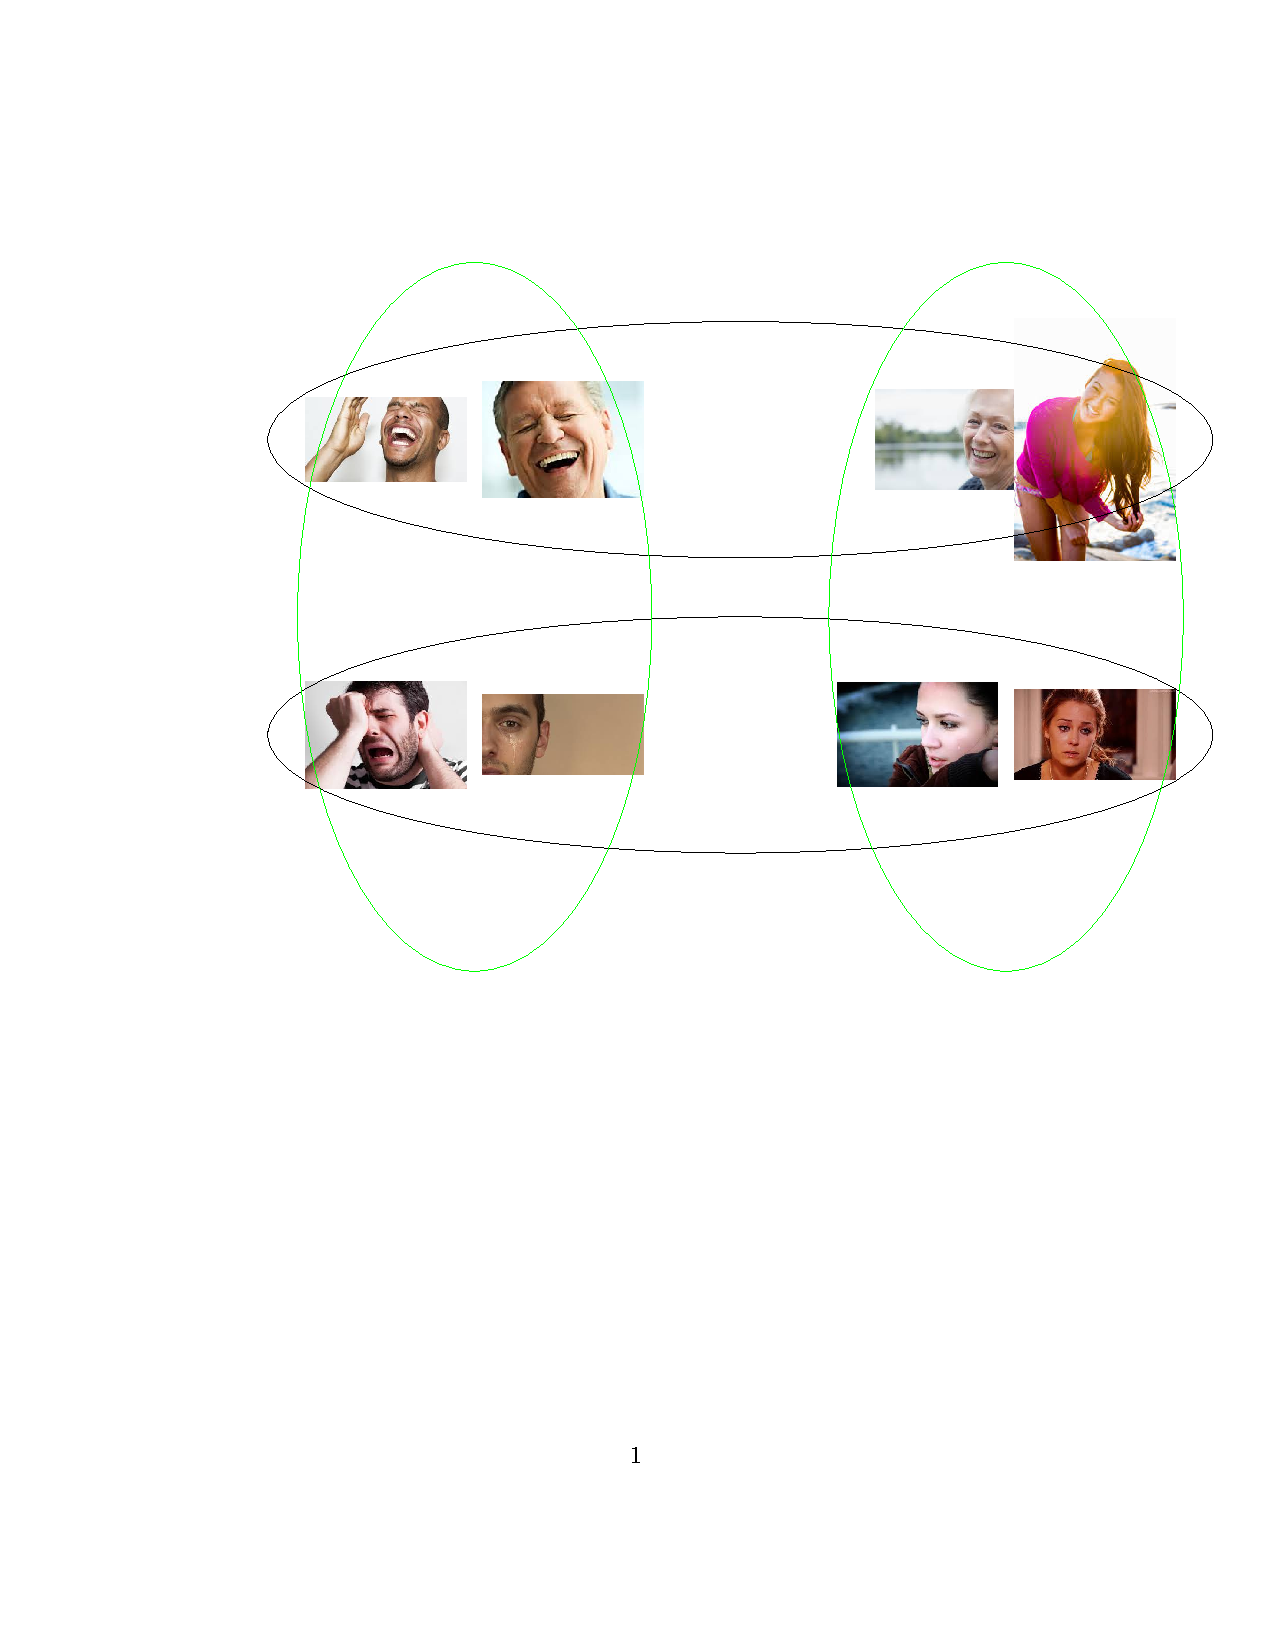
\includegraphics[trim={100 320 30 120},clip,width=0.8\textwidth]{figures/incompatible.pdf}
	\end{center}
	\caption{Under-specificity in clustering.}
	\label{fig:laugh-cry}
	\end{figure}

	Lets consider a concrete example. Consider a dataset of images of faces of people (both male and female) with different emotions (eg. laughing and crying). This toy dataset is shown in Fig. \ref{fig:laugh-cry}. Now, this dataset has two `correct' $2$-clusterings. One clustering is when the males are in one cluster and the females are in another.. Second clustering is when people laughing are in one cluster and the people crying are in another cluster. Both these are reasonable choices. 
	
	However, without extra information, the algorithm doesn't know which one it should prefer. It is possible that the clustering outputted by the algorithm is not what the `user' or the application desired. This is problem of under-specificity which arises whenever multiple solutions are possible. 
\end{itemize}

\section{Concrete questions}
Despite the challenges, clustering algorithms like $k$-means, $k$-median algorithms have been employed successfully in practice. Some applications include cancerous data detection, search engines etc. \cite{wang2005comparison,liu2007clustering}. 

Any satisfactory theory of clustering must examine and explain this gap between theory and practice. In particular

\begin{itemize}
	\item Under what conditions on data are $k$-means or $k$-median optimization problems easy to solve?
	\item Is it possible to have datasets on which popular clustering approaches fail but the proposed algorithm works?
	\item Are there clustering algorithms which take the structure of the data into account? When do these approaches work and when do they fail?
	\item How do you extract domain knowledge to better define the clustering task?
\end{itemize}

These are some of the questions that we would like to answer in our research. We have already made some progress on some of these questions. 

\section{Structure of the proposal}
In Chapter \ref{RLW}, we review some of the previous approaches in dealing with the challenges of clustering. In Chapter \ref{METHOD}, we introduce our notation and some definitions which will be used in the remainder of the proposal. In Chapters \ref{ANALYSIS} and \ref{SSC}, we discuss the approach we have taken to deal with the challenges in clustering. In Chapter \ref{FUTURE}, we discuss the avenues for future work. 








%============================================
\chapter{Related Work}
\label{RLW}
%=============================================
\section{Common previous approaches}
As discussed in Chapter \ref{introduction:challenges}, the most common approach to solving the clustering problem is to pose it as an optimization problem. Some of the examples include $k$-means optimization, $k$-median optimization, $k$-medoids etc. Below, we give a more formal definition of the $k$-means problem. 

\begin{definition}[$k$-means optimization]
Let $(\mb M, d)$ be a metric space. Given a finite set $\mc X \subseteq \mb M$ and $k$. Let $\mc C = \{C_1, \ldots. C_k\}$ be a partition of $\mc X$ into $k$ disjoint subsets. The goal is to find:
$$\argmin_{\mc C} \sum_{i=1}^k \sum_{x \in C_i} d^2(x, c_i)$$
where $c_i \in \mb M$ is the mean of all the points in $C_i$.  
\end{definition}

It has been shown that solving this optimization is NP-Hard \cite{dasgupta2008hardness}. In practice, heuristics are used to solve the minimization problem. The most popular is the Lloyd's algorithm \cite{lloyd1982least}. This algorithm has been used successfully on some clustering applications like cancerous data detection, search engines etc. \cite{wang2005comparison,liu2007clustering}. However, it is known that the Lloyd's algorithm can get stuck at local minima. It can sometimes even produce counter-intuitive clusterings \cite{mirkes2011k}. Similarly, other problems like $k$-median have also been shown to be NP-Hard \cite{megiddo1984complexity}.  

Another question that people have investigated is that ``Is it possible to find an approximation to the optimal solution?". In many cases, the answer to this question is also negative. $K$-Means is NP-Hard to approximate (Awasthi et. al \cite{awasthi2015hardness}). Constant factor approximation algorithms are known for the $k$-median problem. Arya et. al \cite{arya2004local} provide a $(3+\epsilon)$ approximation to the $k$-median cost. If the underlying metric is Euclidean, Kolliopoulos et. al \cite{kolliopoulos1999nearly} provide a $(1+\epsilon)$-approximation to the $k$-median cost. 

In majority of the cases, due to computational hardness, people have to rely on heuristics to solve the clustering problem. These heuristics have no performance guarantees and can often get stuck at local minima. 

\section{Dealing with computational hardness}
Despite the negative hardness results, clustering is applied successfully in practice. Researchers have examined this gap between theory and practice. One hypothesis that has recently gained traction is that ``Clustering is difficult only when it doesn't matter" or the CDNM thesis \cite{daniely2012clustering}. 

This means that the data on which clustering algorithms are computationally expensive do not occur in practice. Researchers have characterized such data sets by defining notions of \textit{clusterable} data. They then propose efficient clustering algorithms for these {\em nice} datasets.

Various notions of clusterability have been considered in the literature. Bilu et. al \cite{bilu2012stable} considered the problem of max-cut clustering of graphs. They defined an input instance to be `stable' if the optimal clustering doesn't change under small multiplicative perturbations. They designed an efficient clustering algorithm for $O(\sqrt{|\mc X|})$-resilient instances. 

Continuing the same line of work, Awasthi et. al \cite{awasthi2012center} defined the notion of $\alpha$-center proximity. Informally speaking, a clustering has $\alpha$-center proximity if any point is $\alpha$ times closer to its own cluster center than to any other center. Bigger the $\alpha$, more is the separation. If the $k$-median optimal solution satisfies $(\alpha > 3)$-center stability then Awasthi et. al \cite{awasthi2012center} give an efficient algorithm to find the optimal. Balcan et. al \cite{balcan2012clustering} then improved this result to $\alpha > \sqrt{2}+1$. The problem is NP-Hard for $\alpha < 2$ \cite{ben2014data}. 

Observe that the results discussed above assume that the entire input dataset has the niceness property. This assumption is very strict and unrealistic. A natural relaxation is to allow few points which do not have the niceness property. Such points are referred to as \textit{noise}. Balcan et. al \cite{balcan2012clustering} considered an input which has $\alpha$-center proximity except for an $\epsilon$ fraction of the points. For $\alpha > 2 + \sqrt{7}$, they were then able to find a $1+O(\epsilon)$-approximation to the cost of the $k$-median optimal solution. 

Ben-David et. al \cite{ben2014clustering} introduced a somewhat-related notion of $\lambda$-center separation. They showed that if the input has this property then they can convert any clustering algorithm to one which is robust to noise. Their framework is very general. They can `robustify' any center-based clustering algorithm. However, they require very strong conditions on the separability of the data as well as noise. 

In a different line of work, Ostrovsky et. al \cite{ostrovsky2006effectiveness} defined a notion of $\epsilon$-separatedness. An input satisfies this niceness property if the cost of the optimal $k$-clustering is $\epsilon^2$ times less than the cost of the optimal $(k-1)$-clustering. Ostrovsky et. al \cite{ostrovsky2006effectiveness} propose a variant of the Lloyd's algorithm. They show that if the input has $\epsilon$-separatedness then with high probability their algorithm finds a near-optimal $k$-means clustering.

Awasthi et. al \cite{awasthi2010stability} introduce a notion of \textit{weak deletion stability} (WDS). Informally speaking, it says that a clustering has $(1+\alpha)$-WDS if deleting one of the clusters increases the cost by a factor of atleast $(1+\alpha)$. If the data has this property then they propose an algorithm which finds a $(1+\epsilon)$-approximation to the cost of the optimal clustering in $O(k |\mc X|^{poly(1/\epsilon , 1/\alpha)})$ time. 

\section{Dealing with under-specificity}
As discussed in Chapter \ref{introduction:challenges}, another major challenge in clustering is under-specificity. Same dataset can have multiple `correct' clusterings. A clustering which is correct (suitable) for one application maybe counter-intuitive for another application. Without knowledge of the intended application, many popular clustering algorithms would fail on a lot of applications. This is probably one of the reasons that clustering is not as widely used as it should be.  In this section, we will discuss two approaches on dealing with under-specificity. 

\subsection{Multiple solutions} 
One simple approach is to allow the algorithm to output multiple solutions. A hierarchical clustering tree is one way to efficiently represent different `feasible' clusterings of the input dataset. The clustering of choice can then be found by efficiently searching over the different prunings of the tree. This approach has been taken Balcan et. al \cite{balcan2012clustering}. 

Another approach is to allow the algorithm to output a small list of what it considers feasible or good clusterings. Note that any list of size $O(|\mc X|^k)$ can output all the partitions of the dataset. Hence, any such list should have size polynomial in $k$ and $|\mc X|$.
   
\subsection{User interaction}
A more interesting approach is to incorporate domain expertise by allowing the algorithm to interact with or get advice from a user. This framework is sometimes referred to as \textbf{semi-supervised clustering}. The advice is aimed at getting rid of the ambiguity in clustering. 

This question has been addressed mainly in some application-oriented works. The algorithm gets as input, a dataset $\mc X$. In addition, \textit{link/do-not-link} constraints are also provided by the user. These constraints basically say that a particular pair of input instances should (or shouldn't) belong to the same cluster. Basu et. al \cite{basu2002semi} used these constraints to help guide the choice of initial centers in the Lloyd algorithm. 

Another way to incorporate supervision is to assume that the data is generated from a particular distribution. The task is then to estimate the parameters of this distribution (\cite{basu2004probabilistic, kulis2009semi}). Ashtiani et. al \cite{ashtiani2015representation} incorporated supervision by asking the user or expert to cluster a small subset of the dataset. Using this information, their algorithm tries to infer the `true' clustering. 

Balcan et. al \cite{balcan2008clustering} considered an interactive model of clustering. Their framework works as follows. The expert is provided with the current clustering. The expert then responds back by suggesting to either split a cluster or merge two clusters. The authors investigate the computational and query complexity of this problem. 









%======================================================================
\chapter{Preliminaries}
\label{METHOD}
%======================================================================

Let the metric space be $(\mb M, d)$. We are given a finite set $\mc X \subseteq \mb M$. A $k$-clustering of $\mc X$, denoted by $\mc C_{\mc X} = \{C_1, \ldots, C_k\}$, is a partition of $\mc X$ into $k$ disjoint subsets. Given points (or centers) $c_1, \ldots, c_k \in \mb M$. The $k$-clustering induced by these points assigns each point in $\mc X$ to its nearest center $c_i$. Such a clustering is also known as center-based clustering.

\begin{definition}[$r(\mc C_{\mc X}), m(\mc C_{\mc X})$]
Given clustering $\mc C_{\mc X} = \{C_1, \ldots, C_k\}$ induced by centers $c_1, \ldots, c_k \in \mb M$, we define 
\begin{align*}
&m(\mc{C}_{\mc{X}}) = \min_i |C_i|\\
&r(\mc{C}_{\mc{X}}) = \max_i \thinspace r(C_i)
\end{align*}
where the radius of a set $\mc A$ given a center $c$ is defined as $\max_{x \in \mc A} d(x, c)$.
\end{definition}

\noindent Consider any center-based clustering. There are two possibilities. In the first case, the centers $c_1, \ldots, c_k$ can be arbitrary points in the metric space $\mb M$. This is known as the \textbf{steiner} setting. In the second case, the centers are restricted to be members of the dataset $\mc X$. This is the \textbf{proper} setting. 

\section{Clusterability notions}
As discussed in previous chapters, various clusterability notions have been considered to explain the success of clustering algorithms. The intention is to show that clustering is easy if the data has this nice property or the data is clusterable. In this section, we discuss some of the notions which have considered and some which we have introduced.

\subsection{Center proximity}
\begin{definition}[$\alpha$-center proximity \cite{awasthi2012center}]
\label{defn:alphacp}
A clustering $\mc C_{\mc X} = \{C_1, \ldots, C_k\}$ satisfies $\alpha$-center proximity w.r.t $\mc X$ and $k$ if there exist centers $c_1, \ldots, c_k \in \mb M$  such that the following holds. For all $x \in C_i$ and $i\neq j$, $$\alpha d(x, c_i) < d(x, c_j)$$
\end{definition}
The notion of center proximity was introduced by Awasthi et. al \cite{awasthi2012center}. It says that each point is $\alpha$-times closer to its own cluster center than to any other centers. Note that this definition works in noise-less case. That is, it assumes that all the points in the input $\mc X$ satisfy the niceness property. A more relaxed version, considered by Balcan et. al \cite{balcan2012clustering}, is when all except an $\epsilon$ fraction of input points satisfy this definition. 

Below, we consider an even more relaxed version which we call $(\alpha, \eta)$-center proximity. It says that the input has a subset $\mc S \subseteq \mc X$ which satisfies the niceness property. Also, the remaining part of the dataset (or noise) is `sparse'. Informally, this means that any ball in our metric space $\mb M$ has few points from $\mc X \setminus \mc S$. 

\begin{definition}[$(\alpha, \eta)$-center proximity]
\label{def:alphaeta}
Given $\mc S \subseteq \mc X$, a clustering $\mc C_{\mc S} = \{S_1, \ldots, S_k\}$ has $(\alpha, \eta)$-center proximity w.r.t $\mc X, \mc S$ and $k$ if there exists centers $s_1, \ldots, s_k \in \mb M$  such that the following holds.

\begin{itemize}
\label{defn:alphacpnoise}	
\item[$\diamond$] {\bf $\alpha$-center proximity}: For all $x \in S_i$ and $i\neq j$, $\thinspace\alpha d(x, s_i) < d(x, s_j)$
\item[$\diamond$]{\bf $\eta$-sparse noise}: For any ball $B$, $r(B)\leq \eta \thinspace r(\mc{C}_{\mc S}) \implies |B\cap (\mc X\setminus \mc S)| < \frac{m(\mc C_{\mc S})}{2}$
\end{itemize}
\end{definition}

\subsection{Center Separation}
\begin{definition}[$\lambda$-center separation \cite{ben2014clustering}]
\label{defn:lambdacs}
A clustering $\mc C_{\mc X} = \{C_1, \ldots, C_k\}$ has $\lambda$-center separation w.r.t $\mc X$ and $k$ if there exists centers $c_1, \ldots, c_k \in \mb M$ such that $\mc C_{\mc X}$ is the clustering induced by these centers and the following holds. For all $i\neq j$, $$d(c_i, c_j) > \lambda r(\mc{C}_{\mc{X}})$$
\end{definition}

Same as before, we consider a relaxed version of this definition which we call $(\lambda, \eta)$-center proximity. The input has a subset $\mc S \subseteq \mc X$ which satisfies center separation while the remaining part is sparse. 

\begin{definition}[$(\lambda, \eta)$-center separation]
Given $\mc S \subseteq \mc X$, a clustering $\mc C_{\mc S}$ has $(\lambda, \eta)$-center separation w.r.t $\mc X, \mc S$ and $k$ if there exists centers $s_1, \ldots, s_k \in \mb M$ such that $\mc C_{\mc X}$ is the clustering induced by these centers and the following holds.

\begin{itemize}
\label{defn:lambdacsnoise}
\item[$\diamond$] {\bf $\lambda$-center separation}: For all $i\neq j$, $\thinspace d(s_i, s_j) > \lambda r({\mc C}_{\mc S})$
\item[$\diamond$]{\bf $\eta$-sparse noise}: For any ball $B$, $r(B)\leq \eta \thinspace r(\mc{C}_{\mc S}) \implies |B\cap (\mc X\setminus \mc S)| < \frac{m(\mc C_{\mc S})}{2}$
\end{itemize}
\end{definition}

\subsection{Margin assumption}
\begin{table}[]
\centering
\caption{Known results for $\alpha$-center proximity}
\label{table:alphacp}
\begin{tabular}{lll}
\cline{2-3}
\multicolumn{1}{l|}{} & \multicolumn{1}{l|}{Euclidean} & \multicolumn{1}{l|}{General Metric} \\ \hline
\multicolumn{1}{|l|}{\begin{tabular}[c]{@{}l@{}}Centers \\ from data\end{tabular}} & \multicolumn{1}{l|}{\begin{tabular}[c]{@{}l@{}}Upper bound : $\sqrt{2}+1$  \cite{balcan2012clustering}\\ Lower bound : ?\end{tabular}} & \multicolumn{1}{l|}{\begin{tabular}[c]{@{}l@{}}Upper bound : $\sqrt{2}+1$  \cite{balcan2012clustering}\\ Lower bound : 2 \cite{ben2014data}\end{tabular}} \\ \hline
\multicolumn{1}{|l|}{\begin{tabular}[c]{@{}l@{}}Unrestricted \\ Centers \end{tabular}} & \multicolumn{1}{l|}{\begin{tabular}[c]{@{}l@{}}Upper bound : $2+\sqrt{3}$ \cite{awasthi2012center}\\ Lower bound : ?\end{tabular}} & \multicolumn{1}{l|}{\begin{tabular}[c]{@{}l@{}}Upper bound : $2+\sqrt{3}$ \cite{awasthi2012center}\\ Lower bound : 3 \cite{awasthi2012center}\end{tabular}} \\ \hline
 &  & 
\label{table:alphacenter}
\end{tabular}
\end{table}

\begin{definition}[$\gamma$-margin]
\label{defn:gammamargin}
A clustering $\mc C_{\mc X} = \{C_1, \ldots, C_k\}$ has $\gamma$-margin w.r.t $\mc X$ and $k$  if there exists centers $c_1, \ldots, c_k \in \mb M$ such that $\mc C_{\mc X}$ is the clustering induced by these centers and the following holds. For all $x \in C_i$ and $y \in {\mc X} \setminus C_i$,
$$\gamma d(x, \mu_i) < d(y, \mu_i)$$
\end{definition}

\begin{table}[]
\centering
\caption{Results for $\gamma$-margin}
\label{table:gammamargin}
\begin{tabular}{lll}
\cline{2-3}
\multicolumn{1}{l|}{}                                                                     & \multicolumn{1}{l|}{Euclidean} & \multicolumn{1}{l|}{General Metric}                                                                         \\ \hline
\multicolumn{1}{|l|}{\begin{tabular}[c]{@{}l@{}}Centers \\ from data\end{tabular}}        & \multicolumn{1}{l|}{\begin{tabular}[c]{@{}l@{}}Upper bound : 2 (Thm. \ref{thm:upperCenterData})\\ Lower bound : ? \end{tabular}}    &       \multicolumn{1}{l|}{\begin{tabular}[c]{@{}l@{}}Upper bound : 2 (Thm. \ref{thm:upperCenterData})\\ Lower bound : 2 (Thm. \ref{thm:lowerCenterData})\end{tabular}}           \\ \hline
\multicolumn{1}{|l|}{\begin{tabular}[c]{@{}l@{}}Unrestricted \\Centers \end{tabular}} & \multicolumn{1}{l|}{\begin{tabular}[c]{@{}l@{}}Upper bound : 3 (Thm. \ref{thm:upperCenterMetric})\\ Lower bound : 1.84 (Thm. \ref{A-thm:gammaLower})\\ \end{tabular}}         & \multicolumn{1}{l|}{\begin{tabular}[c]{@{}l@{}}Upper bound : 3 (Thm. \ref{thm:upperCenterMetric})\\ Lower bound : 3 (Thm. \ref{thm:lowerCenterMetric})\\ \end{tabular}} \\ \hline
                                                                                          &                       &    
\label{table:gammamargin}                                                                                                                                                                                                 
\end{tabular}
\end{table}
  
\noindent The margin assumption is closely related to center proximity. From Tables \ref{table:alphacenter} and \ref{table:gammamargin}, it is clear that the results which were obtained in literature using center proximity assumptions can also be obtained using margin assumptions. Also, observe that under margin assumptions, in a lot of cases, the upper and lower bounds are tight. This shows that the margin assumption is a more natural property than center proximity and provides separation of easy and hard instances. 

\section{Same-cluster queries}
We discussed in previous chapters that under-specificity is one of the major challenges in clustering. To get around this problem, one of the approaches has been to incorporate domain knowledge by using some form of weak supervision. In our framework, this is accomplished by the use of same-cluster queries. 

Given a $k$-clustering $\mc C = \{C_1, \ldots, C_k\}$ of some set $\mc X$. A $\mc C$-oracle is a function $f_{\mc C}$ that answers queries according to the clustering $\mc C$.

\begin{definition}[Same-cluster Query]
\label{defn:sameclusterquery}
A same-cluster query asks whether two instances $x_1$ and $x_2$ belong to the same cluster, i.e., 
$$f_{\mc C}(x_1, x_2) = \left\{
	\begin{array}{ll}
		\mbox{true }  & \mbox{if } x_1 \overset{\mc C}{\sim} x_2   \\
		\mbox{false } & otherwise 
	\end{array}
\right. $$
\end{definition} 

Similar to same-cluster queries are, what we call, cluster-assignment queries. In this case, given a single point $x$, the oracle returns the index of the cluster in which $x$ belongs. More formally, 

\begin{definition}[Cluster-assignment Query]
$f_{\mc C}(x) = i \iff x \in C_i$.
\end{definition}

Note that each cluster-assignment query can be replaced by $k$ same-cluster queries. However, often it is more convenient to describe our algorithms and results in terms of cluster-assignment queries. Also, any same-cluster query can be replaced by two cluster assignment queries. Hence, the two query models are equivalent upto a polynomial factor. 

\section{Miscellaneous definitions}
\begin{definition}[$\mc C_{\mc X}$ restricted to a set] Given $\mc S \subseteq \mc X$ and a clustering $\mc C_{\mc X} = \{C_1, \ldots, C_k\}$ of the set $\mc X$. We define $\mc C_{\mc X}$ restricted to the set $\mc S$ as $\mc C_{{\mc X}|_{\mc S}} = \{C_1 \cap S, \ldots, C_k \cap S\}$. 
\end{definition}

\begin{definition}[$\mc C_{\mc X}$ respects $\mc C_{\mc S}$] Given $\mc S \subseteq \mc X$, clusterings $\mc C_{\mc X} = \{C_1, \ldots, C_k\}$ and $\mc C_{\mc S} = \{S_1, \ldots, S_{k'}\}$. We say that $\mc C_{\mc X}$ respects $\mc C_{\mc S}$ if $\mc C_{{\mc X}|_{\mc S}} = \mc C_{\mc S}$.
\end{definition}

\begin{definition}[$\mc T$ or $\mc L$ captures $\mc C_{\mc S}$]Given a hierarchical clustering tree $\mc T$ of $\mc X$ and a clustering $\mc C_{\mc S}$ of $\mc S \subseteq \mc X$.  We say that $\mc T$ captures $\mc C_{\mc S}$ if there exists a pruning $\mc P$ which respects $\mc C_{\mc S}$. 

Similarly, given a list of clusterings $\mc L$ of $\mc X$ and a clustering $\mc C_{\mc S}$ of $\mc S \subseteq \mc X$. We say that $\mc L$ captures $\mc C_{\mc S}$ if there exists a clustering $\mc C_{\mc X} \in \mc L$ which respects $\mc C_{\mc S}$. 
\end{definition}






 
%======================================================================
\chapter{Clustering under Sparse Noise}
\label{ANALYSIS}
%======================================================================
One of the major challenges of clustering is that it is computationally expensive. In Chapter \ref{RLW}, we discussed a recent line of work to address this issue, namely, notions of clusterability. The basic idea is to show that clustering is easy (computationally cheap) if the data has some nice properties. However, lot of these notions are unrealistic. They impose very strict conditions on the input. Such conditions are not likely to occur in real-world situations. 

The reason for this is that adequate attention has not been paid to clusterability notions which handle noise. Previously, researchers have addressed noise robustness in a very limited context, like uniform random noise or worst-case adversarial noise \cite{balcan2012clustering,ackerman2009clusterability}.

In this chapter we will take a different approach. What distinguishes noise from `nice' part of the input data? In many real-world applications, apart from having cohesive subsets, the data also has a ``gray background'' that it is \emph{structureless} or \emph{sparse}. We introduced our notions in Defn. \ref{def:alphaeta} and \ref{defn:lambdacsnoise}. Note that this definition imposes no restriction on the size of the noisy data.  We can handle as many noisy points as possible as long as they are sparse. 

Our approach diverges from previous discussions of clusterable data in yet another aspect. Much of the theoretical research of clustering algorithms views clustering as an optimization problem (which are NP-Hard to solve). Hence, heuristics are used to solve the optimization problem. However, given a large dataset, there is no way to know the cost of the optimal solution or how close the output of the heuristic is to the optimal solution. But the user may have some notion of a meaningful cluster and would be happy if the output `captures' any such nice solution. 

In the next section, we first present algorithm which captures all nice solutions if the input satisfies $(\alpha, \eta)$-center proximity. We then show that if the parameters $\alpha$ or $\eta$ are relaxed, then such results are no longer possible. We do a simialr analysis when the input satisfies $(\lambda, \eta)$-center separation as well.  

\section{Center Proximity}
We study the problem of recovering all $(\alpha, \eta)$-center proximal clusterings of a set $\mc X$. The goal of our algorithm is to produce an efficient representation (hierarchical clustering tree) of all possible $(\alpha, \eta)$-center proximal nice clusterings rather than to output a single clustering or to optimize an objective function.
\begin{itemize}
\item  {\it Positive result under sparse noise} - In Section \ref{section:positiveResultSparseNoise}, we give our main result under sparse noise. If $\alpha \ge 2 + \sqrt{7} \approx 4.6$ and $\eta \ge 1$; for any value of $t$, Alg.~\ref{alg:alphacp} outputs a tree which captures all clusterings $\mc C^*$ (of a subset of $\mc X$) which satisfy $(\alpha, \eta)$-center proximity and $m(C^*)=t$.
\item  {\it Lower bound under sparse noise} - In Section \ref{section:alphaLowerBoundSparse}, we show that if $\alpha \le 2 + \sqrt{3} \approx 3.7$ and $\eta \le 1$ then there is no tree and no list of `small' size ($< 2^{k/2}$) which can capture all clusterings $\mc C$ (of a subset of $\mc X$) which satisfy $(\alpha, \eta)$-center proximity even for a fixed value of the size of the smallest cluster $(m(C) = t)$.
\item {\it Lower bound with arbitrary noise} - In Section \ref{section:alphaLowerBoundArbitrary}, we show that for a given value of a parameter $t$, if $\alpha \le 2\sqrt{2} + 3 \approx 5.8$ and the number of noisy points exceeds $\frac{3}{2}t$ then no tree can capture all clusterings $\mc C$ (of a subset of $\mc X$) which satisfy $\alpha$-center proximity even for fixed $m(\mc C) = t$. Identical result holds for `small' ($<2^{k/2}$) lists if the number of noisy points exceeds $\frac{3k}{2}t$.
\end{itemize} 

\subsection{Positive result under sparse noise}
\label{section:positiveResultSparseNoise}
Given a clustering instance $(\mc X, d)$ and a parameter $t$, we introduce an efficient algorithm which outputs a hierarchical clustering tree $\mc T$ of $\mc X$ with the following property. For every $k$, for every $\mc S \subseteq \mc X$ and for every $k$-clustering $\mc C_{\mc S}$ which satisfies $(\alpha, \eta)$-center proximity (for $\alpha \ge 2 + \sqrt{7}$ and $ \eta \ge 1)$ and $m(\mc C_{\mc S}) = t$, $\mc T$ captures $\mc C_{\mc S}$. It is important to note that our algorithm only knows $\mc X$ and has no knowledge of the set $\mc S$.

Our algorithm has a linkage based structure similar to \cite{balcan2012clustering}. However, our method benefits from a novel {\it sparse distance condition}. We introduce the algorithm in Alg.~\ref{alg:alphacp} and prove its efficiency and correctness in Theorem~\ref{thm:algcptime} and Theorem~\ref{thm:alphacpnoise} respectively. 

\begin{definition}[Sparse distance condition]
	 Given a clustering $\mc C = \{C_1,\\\ldots,C_k\}$ of the set $\mc X$ and a parameter $t$. We say that the ball $B \subseteq \mc X$ satisfies the sparse distance condition w.r.t clustering $\mc C$ when the following holds.
	 
\begin{itemize}
\item $|B| \ge t$.
\item For any $C_i \in \mc C$, if $C_i \cap B \neq \emptyset$, then $C_i \subseteq B$ or $|B \cap C_i| \ge t/2$.
\end{itemize}
\end{definition}

Intuitively, Alg.~\ref{alg:alphacp} works as follows. It maintains a clustering $\mc C^{(l)}$, which is initialized so that each point is in its own cluster. It then goes over all pairs of points $p, q$ in increasing order of their distance $d(p, q)$. If $B(p, d(p,q))$ satisfies the sparse distance condition w.r.t $\mc C^{(l)}$, then it merges all the clusters which intersect with this ball into a single cluster and updates $\mc C^{(l)}$. Furthermore, the algorithm builds a tree with the nodes corresponding to the merges performed so far. We will show that for all $\mc S \subseteq \mc X$ which are $(\alpha, \eta)$-proximal $t$-min nice and for all clusterings $\mc C_S$ which have $(\alpha, \eta)$-center proximity, Alg.~\ref{alg:alphacp} outputs a tree which captures $\mc C_S$.

\begin{algorithm}
	\SetAlgoLined
	\KwIn{$(\mc X, d)$ and $t$}
	\KwOut{A hierarchical clustering tree $T$ of $\mc X$.}
	
\vspace{0.1in}Let $\mc C^{(l)}$ denote the clustering $\mc X$ after $l$ merge steps have been performed. Initialize $\mc C^{(0)}$ so that all points are in their own cluster. That is, $\mc C^{(0)} = \{ \{x\}: x \in \mc X\}$.
	
	Go over all pairs of points $p, q$ in increasing order of the distance $d(p, q)$. If $B = B(p, d(p, q))$ satisfies the sparse distance condition then\\
	\hspace{0.24in}Merge all the clusters which intersect with $B$ into a single cluster.
	
	\vspace{0.1in}Output clustering tree $T$. The leaves of $T$ are the points in dataset $\mc X$. The internal nodes correspond to the merges performed.
\caption{Alg. for $(\alpha, \eta)$-center proximity with parameter $t$}	
\label{alg:alphacp}
\end{algorithm}

%\vspace{-.1in}
\begin{theorem}
\label{thm:alphacpnoise}
Given a clustering instance $(\mc X, d)$ and a parameter $t$. Alg.~\ref{alg:alphacp} outputs a tree $\mc T$ with the following property. For all $k$, $\mc S \subseteq \mc X$ and for all $k$-clusterings $\mc C^*_{\mc S} = \{S_1^*, \ldots, S_k^*\}$ which satisfy $(2+\sqrt{7}, 1)$-center proximity the following holds. If $m(\mc C_{\mc S}^*) = t$ then $\mc T$ captures $\mc C_{\mc S}$.
\end{theorem}

\begin{theorem}
\label{thm:algcptime}
Given clustering instance $(\mc X, d)$ and $t$. Alg.~\ref{alg:alphacp} runs in  $poly(|\mc X|)$.
\end{theorem}

\begin{proof}
Let $n = |\mc X|$. Checking if $B$ satisfies the sparse-distance condition takes $O(n)$ time and hence the algorithm runs in $O(n^3)$ time.
\end{proof}

\subsection{Lower bound under sparse noise}
\label{section:alphaLowerBoundSparse}
\begin{theorem}
\label{thm:noalgalphacp}
Given the number of clusters $k$ and parameter $t$. For all $\alpha \le 2+\sqrt{3}$ and $\eta \le 1$ there exists a clustering instance $(\mc X, d)$ such that any clustering tree $\mc T$ of $\mc X$ has  the following property. There exists $\mc S \subseteq \mc X$ and clustering $\mc C_{\mc S}$ which satisfies $(\alpha, \eta)$-center proximity and $ m(\mc C_{\mc S}) = t$ but $\mc T$ doesn't capture $\mc C_{\mc S}$.
\end{theorem}

\begin{theorem}
\label{thm:nolistalphacp}
Given the number of clusters $k$ and parameter $t$. For all $\alpha \le 2+\sqrt{3}$, $\eta \le 1$ there exists $(\mc X, d)$ such that any list $\mc L$ (of clusterings of $\mc X$) has  the following property. If $|\mc L| < 2^{\frac{k}{2}}$ then there exists $\mc S \subseteq \mc X$ and clustering $\mc C_{\mc S}$ which satisfies $(\alpha, \eta)$-center proximity and $ m(\mc C_{\mc S}) = t$ but $\mc L$ doesn't capture $\mc C_{\mc S}$.
\end{theorem}

\subsection{Lower bound under arbitrary noise}
\label{section:alphaLowerBoundArbitrary}

\begin{theorem}
\label{thm:nosparsealg}
Given the number of clusters $k$ and a parameter $t$. For all $\alpha < 2\sqrt 2 + 3$ there exists $(\mc X, d)$ such that any clustering tree $\mc T$ of $\mc X$ has the following property. There exists $\mc S \subseteq \mc X$ and there exists clustering $\mc C_{\mc S}$ which satisfies $\alpha$-center proximity such that $m(\mc C_{\mc S}) = t$ and the following holds. If $|\mc X \setminus \mc S| \ge \frac{3t(\mc C_{\mc S})}{2}+5$, then $\mc T$ doesn't capture $\mc C_{\mc S}$.
\end{theorem}

\begin{theorem}
\label{thm:nosparselistalphacp}
Given the number of clusters $k$ and parameter $t$. For all $\alpha \le 2+\sqrt{2}+3$ there exists $(\mc X, d)$ such that any list $\mc L$ (of clusterings of $\mc X$) has  the following property. There exists $\mc S \subseteq \mc X$ and there exists clustering $\mc C_{\mc S}$ which satisfies $\alpha$-center proximity such that $m(\mc C_{\mc S}) = t$ and the following holds. If $|\mc L| < 2^{\frac{k}{2}}$ and $|\mc X \setminus \mc S|\ge \frac{k}{2}(\frac{3t(\mc C_{\mc S})}{2}+5)$, then $\mc L$ doesn't capture $\mc C_{\mc S}$.
\end{theorem}


\section{Center Separation}
In this section, we study the problem of recovering $(\lambda, \eta)$-center separated clusterings of a set $\mc X$, in the presence of noise. Here is a more precise overview of the results of this section:
\begin{itemize}
\item  {\it Positive result under sparse noise} - In Section \ref{section:lambdaPositiveResultSparseNoise}, we show that if $\lambda \ge 4$ and $\eta \ge 1$; for any value of parameters $r$ and $t$, Alg.~\ref{alg:lambdacs} outputs a clustering which respects all clusterings $\mc C^*$ (of a subset of $\mc X$) which satisfies $(\lambda, \eta)$-center proximity and $m(C^*)=t$ and $r(C^*) = r$.
\item  {\it Lower bound under sparse noise} - In Section \ref{section:lambdaLowerBoundSparse}, we show that, if $\lambda < 4$ and $\eta \le 1$ then there is no tree and no list of `small' size ($<2^{k/2}$) which can capture all clusterings $\mc C$ (of subset of $\mc X$) which satisfy $(\lambda, \eta)$-center proximity even for fixed values of the size of the smallest cluster $(m(C) = t)$ and maximum radius ($r(C) = r$).
\item {\it Lower bound with arbitrary noise} - In Section \ref{section:lambdaLowerBoundArbitrary}, we show that for a given value of parameters $r$ and $t$, if $\lambda \le 6$ and the number of noisy points exceeds $\frac{3}{2}t$ then no tree can capture all clusterings $\mc C$ (of a subset of $\mc X$) which satisfy $\lambda$-center separation even for fixed $m(\mc C) = t$ and $r(\mc C) = r$. Identical result holds for `small' ($<2^{k/2}$) lists if the number of noisy points exceeds $\frac{3k}{2}t$.
\end{itemize}

\subsection{Positive result under sparse noise}
\label{section:lambdaPositiveResultSparseNoise}
We are given a clustering instance $(\mc X, d)$ and parameters $r$ and $t$. Our goal is to output a clustering $\mc C_{\mc X}$ which has the following property. For every $k$, for every $\mc S \subseteq \mc X$ and for every $k$-clustering $\mc C_{\mc S}$ which satisfies $(\lambda, \eta)$-center separation, the clustering $\mc C_{\mc X}$ restricted to $\mc S$ equals $\mc C_{\mc S}$. 

In the next section, we propose a clustering algorithm (Alg.~\ref{alg:lambdacs}) and prove (Theorem~\ref{thm:lambdacsnoise}) that our algorithm indeed achieves the above mentioned goal (under certain assumptions on the parameters $\lambda$ and $\eta$). It is important to note that our algorithm only knows $\mc X$ and has no knowledge of the set $\mc S$. 

Intuitively, Alg.~\ref{alg:lambdacs} works as follows. In the first phase, it constructs a list of balls which have radius at most $r$ and contain at least $t$ points. It then constructs a graph as follows. Each ball found in the first phase is represented by a vertex. If two balls have a `large' intersection then there is an edge between the corresponding vertices in the graph. We then find the connected components in the graph which correspond to the clustering of the original set $\mc X$. 

\begin{algorithm}[!ht]	
	\KwIn{$(\mc X, d), t$ and $r$}
	\KwOut{A clustering $\mc C$ of the set $\mc X$.}
	
	\vspace{0.1in}\textbf{Phase 1}\\
	Let $\mc L$ denote the list of balls found so far. Initialize $\mc L$ to be the empty set. $\mc L = \emptyset$.
	
	Go over all pairs of points $p, q \in \mc X$ in increasing order of the distance $d(p, q)$. Let $B := B(p, d(p, q))$. If $|B| \ge t$ and $r(B) \le r$ then
	
	\hspace{0.24in}$\mc L = \mc L \thinspace\cup B$
	
	\vspace{0.1in}Output the list of balls $\mc L = \{B_1, \ldots, B_l\}$ to the second phase of the algorithm.
	
	\vspace{0.1in}\textbf{Phase 2}\\
	Construct a graph $G = (V, E)$ as follows. $V = \{v_1, v_2, \ldots, v_l\}$. If $|B_i \cap B_j| \ge t/2$ then construct an edge between $v_i$ and $v_j$.
	
	Find connected components ($G_1, \ldots, G_{k}$) in the graph $G$. 
	
	Merge all the points in the same connected component together to get a clustering $\mc C = \{C_1, \ldots, C_k\}$ of the set $\mc X$.
	
	Assign $x \in \mc X \setminus \mc \cup_i B_i$ to the closest cluster $C_i$. That is, $i := \argmin\limits_{j\in [k]} \min\limits_{y \in C_j}d(x, y)$. Output $\mc C$. 
\caption{Alg. for $(\lambda, \eta)$-center separation with parameters $t$ and $r$}
\label{alg:lambdacs}
\end{algorithm}
\vspace{-.1in}
\begin{theorem}
\label{thm:lambdacsnoise}
Given a clustering instance $(\mc X, d)$ and parameters $r$ and $t$. For every $k$, for every $\mc S \subseteq \mc X$ and for all $k$-clusterings $\mc C^*_{\mc S} = \{S_1^*, \ldots, S_k^*\}$ which satisfy $(4, 1)$-center separation such that $ m(\mc C_{\mc S}^*) = t$ and $r(\mc C_{\mc S}^*) = r$, the following holds. Alg.~\ref{alg:lambdacs} outputs a clustering $\mc C_{\mc X}$ such that $\mc C_{\mc X}|_{\mc S} = \mc C_{\mc S}^*$.
\end{theorem}

\begin{theorem}
\label{thm:alglambdacstime}
Given $(\mc X, d)$ and parameters $r$ and $t$. Alg.~\ref{alg:lambdacs} runs in $poly(|\mc X|)$.
\end{theorem}

\begin{proof}
Let $n = |\mc X|$. Phase 1 of Alg.~\ref{alg:lambdacs} runs in $O(n^2)$ time. Phase 2 gets a list of size $l$. Constructing $G$ and finding connected components takes $O(l^2)$ time. Hence, the algorithm runs in $O(n^2)$ time.
\end{proof}


\subsection{Lower bound under sparse noise}
\label{section:lambdaLowerBoundSparse}
\begin{theorem}
\label{thm:noalglambdacs}
Given the number of clusters $k$ and parameters $r$ and $t$. For all $\lambda < 4$ and $\eta \le 1$, there exists a clustering instance $(\mc X , d)$ such that any clustering tree $\mc T$ of $\mc X$ has the following property. There exists $\mc S \subseteq \mc X$ and a $k$-clustering $\mc C_{\mc S} = \{S_1, \ldots, S_k\}$ which satisfies $(\lambda, \eta)$-center separation such that $m(\mc C_{\mc S}) = t$ and $r(\mc C_{\mc S}) = r$, but $\mc T$ doesn't capture $\mc C_{\mc S}$.
\end{theorem}

\begin{theorem}
\label{thm:nolistlambdacs}
Given the number of clusters $k$ and parameters $r$ and $t$. For all $\lambda \le 4$ and $\eta \le 1$ there exists a clustering instance $(\mc X, d)$ such that any list $\mc L$ (of clusterings of $\mc X$) has  the following property. If $|\mc L| < 2^{\frac{k}{2}}$ then there exists $\mc S \subseteq \mc X$ and clustering $\mc C_{\mc S}$ which satisfies $(\lambda, \eta)$-center separation and $ m(\mc C_{\mc S}) = t$ and $r(\mc C_{\mc S}) = r$, but $\mc L$ doesn't capture $\mc C_{\mc S}$.
\end{theorem}


\subsection{Lower bound with arbitrary noise}
\label{section:lambdaLowerBoundArbitrary}

\begin{theorem}
\label{thm:nosparselambdaalg}
Given the number of clusters $k$ and parameters $r$ and $t$. For all $\lambda < 6$, there exists a clustering instance $(\mc X , d)$ such that any clustering tree $\mc T$ of $\mc X$ has the following property. There exists $\mc S \subseteq \mc X$ and there exists $k$-clustering $\mc C_{\mc S}$ which satisfies $\lambda$-center separation such that $m(\mc C_{\mc S}) = t$, $r(\mc C_{\mc S}) = r$ and the following holds. If $|\mc X\setminus \mc S|\ge \frac{3t}{2}+5$, then $\mc T$ doesn't capture $\mc C_{\mc S}$ .
\end{theorem}

\begin{theorem}
\label{thm:nosparselistlambdacs}
Given the number of clusters $k$ and parameters $r$ and $t$. For all $\lambda \le 6$ there exists $(\mc X, d)$ such that any list $\mc L$ (of clusterings of $\mc X$) has the following property. There exists $\mc S \subseteq \mc X$ and there exists clustering $\mc C_{\mc S}$ which satisfies $\lambda$-center separation such that $m(\mc C_{\mc S}) = t$, $r(\mc C_{\mc S}) = r$ and the following holds. If $|\mc L| < 2^{\frac{k}{2}}$ and $|\mc X \setminus \mc S|\ge \frac{k}{2}(\frac{3t(\mc C_{\mc S})}{2}+5)$, then $\mc L$ doesn't capture $\mc C_{\mc S}$.
\end{theorem}










%======================================================================
\chapter{Semi-supervised Clustering}
\label{SSC}
%======================================================================
One of the challenge in clustering is under-specificity. The same dataset can admit multiple solutions depending upon the intended application. One approach to handle this issue is to incorporate domain knowledge via weak human supervision. Chapter \ref{RLW} discusses some of the approaches that researchers have taken to tackle this issue. Most of the approaches were mostly application oriented. The merge-split framework of Balcan et. al \cite{balcan2008clustering} did answer some theoretical questions but was somewhat unrealistic.

In this chapter, we introduce a new framework of human-supervised clustering via same-cluster queries (Defn. \ref{defn:sameclusterquery}). An expert (or an oracle) is given two points and should answer whether the two points belong in the same or different cluster. This work has the potential for a lot of practical applications. Considering the clustering problem in a medical domain. While a doctor can't be expected to evaluate the clustering of a big dataset (as required in the merge-split framework), it is very reasonable to give him a few pairs of patients and ask if they belong to the same cluster or not (depending upon his application).

Another surprising result is that access to few such answers can turn an otherwise NP hard clustering problem into a feasible one. We are not aware of such results in other domains. This result has the potential for applications in other domains of computer science. 

\section{Clustering with same-cluster queries}
\label{section:clusteringWithQuery}

In this section we provide an efficient algorithm for clustering with queries. We assume that the oracle (or expert or human or user) has clustering in his mind which satisfies the $\gamma$-margin property (Defn. \ref{defn:gammamargin}). In addition the center of each cluster is the center of mass of the points in that cluster. Note that our algorithm, not only makes use of same-cluster queries but also cluster-assignment queries.  As discussed in Chapter \ref{METHOD}, the two are equivalent upto a factor of $k$. The use of cluster-assignment queries is mainly to make the algorithm description simpler.

Our algorithm does the following. In the first phase, it tries to estimate the center of one of the clusters (say $C_p$). It does so by the help of cluster-assignment queries. In the second phase, the algorithm then tries to estimate the radius of $C_p$. Here, the algorithm makes use of the $\gamma$-margin property of the instances. After estimating the radius, the algorithm is able to recover all the points in the cluster $C_p$. It then deletes $C_p$ and repeats the process. 


\RestyleAlgo{boxruled} 
\SetAlgoNoLine
\begin{algorithm}
 \KwIn{Clustering instance $\mc X$, oracle $\mc O$, the number of clusters $k$ and parameter $\delta \in (0, 1)$}
 \KwOut{A clustering $\mc C$ of the set $\mc X$}

 \vspace{0.5em} $\mc C = \{\}$,
 $\mc S_{1} = \mc X$,
 $\eta = \beta \frac{\log k + \log(1/\delta)}{(\gamma-1)^4}$\\
 \For{$i = 1$ to $k$}{
 	\vspace{0.5em}\textbf{Phase 1}\\
 	$l = k \eta + 1$\;
	$Z \sim U^l[\mc S_i]$    \mbox{       } //   Draws $l$ independent elements from $\mc S_i$ uniformly at random\\
	For $1 \le t \le i$,\\
             \mbox{            } $Z_t = \{x \in Z : {\mc O}(x)= t\}.$ \mbox{    } //Asks cluster-assignment queries about the members of $Z$\\
    % let $Z_t \subseteq \mc Z$ be the set of points with label $i$. That is, \begin{center}$A_t = \{x \in \mc Z : x \in C_t\}.$\end{center} 
%	Choose any $Z_p$ such that $|Z_p| > \eta$.\\
$p = \argmax_t |Z_t|$\\
	$\mu_p' := \frac{1}{|Z_p|}\sum_{x \in Z_p} x$.\\

	\vspace{0.5em}\textbf{Phase 2}\\
    // We know that there exists $r_i$ such that $\forall x\in {\mc S_i}$, $x\in C_i \Leftrightarrow d(x, \mu^\prime_i)< r_i$.\\ 
    // Therefore, $r_i$ can be found by simple binary search\\
    
	$\widehat{\mc S_i}$ = Sorted$(\{\mc S_i\})$ \mbox{       }// Sorts elements of $\{x: x\in \mc S_i\}$ in increasing order of $d(x, \mu_p')$.\\    
	 $r_i = $ BinarySearch$(\widehat{\mc S_i})$ \mbox{      } //This step takes up to $O(\log|{\mc S_i}|)$ same-cluster queries\\


%Binary search over $\widehat{\mc S_i}$, to find an index $idx$ such that $b_{idx} \in C_p$ and $b_{idx+1} \not\in C_p$. (This step involves making queries to the oracle $\mc O$).\\ %We will later prove that $d(b_{idx}, c_p') = \max_{x \in C_p}d(x, c_p')$.
	$C_p' = \{x \in \mc S_i: d(x, \mu_p') \le r_i\}$.\\
	$S_{i+1} = S_{i}\setminus C_p'$.\\
	$\mc C = \mc C \cup \{C_p'\}$
 }
 \label{alg:steinerQueryPositive}
 \caption{Algorithm for $\gamma(> 1)$-margin instances with queries}
\end{algorithm}


\begin{theorem}
\label{thm:steinerQueryPositive}
Let $(\mc X, d, C)$ be a clustering instance, where $C$ is center-based and satisfies the $\gamma$-margin property. Let $\mu_i$ be the center of mass of $C_i$.
%Given a clustering instance $(\mc X, d)$ in some metric space $M$. Let $\mc C_{\mc X} = \{C_1, \ldots, C_k\}$ be a clustering of $\mc X$ induced by centers $\mu_1, \ldots, \mu_k \in M$ which satisfies $\gamma$-margin and $\mu_i$ is the mean of points in $C_i$. 
Assume $\delta \in (0, 1)$ and $\gamma > 1$. Then with probability at least $1-\delta$, Algorithm \ref{alg:steinerQueryPositive} outputs $C$.
\end{theorem}

\begin{theorem}
\label{thm:steinerQueryPositiveComplexity}
Let the framework be as in theorem \ref{thm:steinerQueryPositive}. Then Algorithm \ref{alg:steinerQueryPositive} 
\begin{itemize}
\item Makes $O\big(k\log n + k^2\frac{\log k + \log (1/\delta)}{(\gamma - 1)^4}\big)$ same-cluster queries to the oracle $\mc O$.
\item Runs in $O\big(kn\log n + k^2\frac{\log k + \log (1/\delta)}{(\gamma - 1)^4}\big)$ time.
\end{itemize}
\end{theorem}

\section{Hardness Results}
\label{section:lowerBounds}

\subsection{Hardness of Euclidean $k$-means with Margin}

Finding $k$-means solution without the help of an oracle is generally computationally hard. In this section, we will show that solving Euclidean $k$-means remains hard even if we know that the optimal solution satisfies the $\gamma$-margin property for $\gamma=\sqrt{3.4}$. In particular, we show the hardness for the case of $k=\Theta(n^\epsilon)$ for any $\epsilon\in (0,1)$.

Given a set of instances $\mc X \subset \mb R ^d$, the $k$-means clustering problem is to find a clustering $\mc C = \{C_1, \ldots, C_k\}$ which minimizes $f(\mc C) = \sum\limits_{C_i} \min\limits_{\mu_i\in {\mb R}^d}\sum\limits_{x\in C_i} \|x - \mu_i \|_2^2$. The decision version of $k$-means is, given some value $L$, is there a clustering $\mc C$ with cost $\le L$? The following theorem is the main result of this section. 

\begin{theorem}
\label{thm:gammaLower}
Finding the optimal solution to Euclidean $k$-means objective function is NP-hard when $k=\Theta(n^\epsilon)$ for any $\epsilon \in (0,1)$, even when the optimal solution satisfies the $\gamma$-margin property for $\gamma = \sqrt{3.4}$.
\end{theorem}

This results extends the hardness result of \cite{ben2014data} to the case of Euclidean 
metric, rather than arbitrary one, and to the $\gamma$-margin condition (instead of the $\alpha$-center proximity there).

\subsubsection{Overview of the proof}

Our method to prove Thm. \ref{thm:gammaLower} is based on the approach employed by \cite{vattani2009hardness}. However, the original construction proposed in \cite{vattani2009hardness} does not satisfy the $\gamma$-margin property. Therefore, we have to modify the proof by setting up the parameters of the construction more carefully. 

To prove the theorem, we will provide a reduction from the problem of Exact Cover by 3-Sets (\textsc{X3C}) which is NP-Complete \cite{garey2002computers}, to the decision version of $k$-means.
%(which given a real value $L$, asks whether a clustering with cost $\le L$ exists).

\begin{definition}[\textsc{X3C}]
Given a set $U$ containing exactly $3m$ elements and a collection $\mc S = \{S_1, \ldots, S_l\}$ of subsets of $U$ such that each $S_i$ contains exactly three elements, does there exist $m$ elements in $\mc S$ such that their union is $U$? 
\end{definition}

We will show how to translate each instance of X3C, $(U,\mc S)$, to an instance of $k$-means clustering in the Euclidean plane, $X$. In particular, $X$ has a grid-like structure consisting of $l$ rows (one for each $S_i$) and roughly $6m$ columns (corresponding to $U$) which are embedded in the Euclidean plane. The special geometry of the embedding makes sure that any low-cost $k$-means clustering of the points (where $k$ is roughly $6ml$) exhibits a certain structure. In particular, any low-cost $k$-means clustering could cluster each row in only two ways; One of these corresponds to $S_i$ being included in the cover, while the other means it should be excluded. We will then show that $U$ has a cover of size $m$ if and only if $X$ has a clustering of cost less than a specific value $L$. Furthermore, our choice of embedding makes sure that the optimal clustering satisfies the $\gamma$-margin property for $\gamma=\sqrt{3.4} \approx 1.84$.


\subsubsection{Reduction design}
Given an instance of X3C, that is the elements $U = \{1, \ldots, 3m\}$ and the collection $\mc S$, we construct a set of points $X$ in the Euclidean plane which we want to cluster. Particularly, $X$ consists of a set of points $H_{l,m}$ in a grid-like manner, and the sets $Z_i$ corresponding to $S_i$. In other words, $X = H_{l,m} \cup (\cup_{i=1}^{l-1} Z_i)$. 

The set $H_{l,m}$ is as described in Fig. \ref{fig:lowerBoundComponent}. The row $R_i$ is composed of $6m + 3$ points $\{s_i, r_{i, 1}, \ldots, r_{i, 6m+1}, f_i\}$. Row $G_i$ is composed of $3m$ points $\{g_{i,1}, \ldots, g_{i, 3m}\}$. The distances between the points are also shown in Fig. \ref{fig:lowerBoundComponent}. Also, all these points have weight $w$, simply meaning that each point is actually a set of $w$ points on the same location.

Each set $Z_i$ is constructed based on $S_i$. In particular, $Z_i = \cup_{j\in [3m]} B_{i,j}$, where $B_{i,j}$ is a subset of $\{x_{i,j},x_{i,j}',y_{i,j},y_{i,j}'\}$ and is constructed as follows: $x_{i,j} \in B_{i,j}$ iff $j \not\in S_i$, and $x_{i,j}' \in B_{i,j}$ iff $j \in S_i$. Similarly,  $y_{i,j} \in B_{i,j}$ iff $j \not\in S_{i+1}$, and $y_{i,j}' \in B_{i,j}$ iff $j \in S_{i+1}$. Furthermore, $x_{i, j}, x_{i,j}^\prime, y_{i,j}$ and $y_{i, j}^\prime$ are specific locations as depicted in Fig. \ref{fig:ZFig}. In other words, exactly one of the locations $x_{i,j}$ and $x_{i,j}^\prime$, and one of $y_{i,j}$ and $y_{i,j}^\prime$ will be occupied. We set the following parameters. 
\vspace{-0.1in}
\begin{align*}
&h = \sqrt{5}, d = \sqrt{6}, \epsilon = \frac{1}{w^2}, \lambda = \frac{2}{\sqrt{3}}h, k = (l-1)3m + l(3m+2)\\
& L_1 = (6m+3)wl, L_2 = 3m(l-1)w, L = L_1 + L_2 - m\alpha, \alpha = \frac{d}{w}-\frac{1}{2w^3}
\end{align*}


  \begin{figure}[!tbp]
  \centering
  \begin{minipage}[b]{0.49\textwidth}
    \resizebox{\linewidth}{!}{\ifdefined\COMPLETE
\else
\documentclass[12pt]{article}
\usepackage{tikz}
\usetikzlibrary{shapes, calc, arrows, through, intersections, decorations.pathreplacing, patterns}

\begin{document}
\fi
\def\alph{$2+\sqrt{5}$}
\begin{tikzpicture}[scale=7]

	\node[label=180:$R_1$] at (0.0,0) {$\diamond$};	
	\node[] at (0.1,0) {$\bullet$};
	\node[] at (0.2,0) {$\bullet$};
	\node[] at (0.3,0) {$\bullet$};
	\node[] at (0.4,0) {$\bullet$};
	\node[] at (0.6,0) {$\ldots$};
	
	\node[] at (0.8,0) {$\bullet$};
	\node[] at (0.9,0) {$\bullet$};
	\node[] at (1.0,0) {$\diamond$};
	
	
	\node[label=180:$G_1$] at (0.0,-0.1) {};	
	\node[] at (0.2,-0.1) {$\circ$};
	\node[] at (0.4,-0.1) {$\circ$};
	\node[] at (0.6,-0.1) {$\ldots$};
	
	\node[] at (0.8,-0.1) {$\circ$};
	
	\node[label=180:$R_2$] at (0.0,-0.2) {$\diamond$};	
	\node[] at (0.1,-0.2) {$\bullet$};
	\node[] at (0.2,-0.2) {$\bullet$};
	\node[] at (0.3,-0.2) {$\bullet$};
	\node[] at (0.4,-0.2) {$\bullet$};
	\node[] at (0.6,-0.2) {$\ldots$};
	
	\node[] at (0.8,-0.2) {$\bullet$};
	\node[] at (0.9,-0.2) {$\bullet$};
	\node[] at (1.0,-0.2) {$\diamond$};
	
	
	
	\node[label=180:$G_{l-1}$] at (0.0,-0.4) {};	
	\node[] at (0.2,-0.4) {$\circ$};
	\node[] at (0.4,-0.4) {$\circ$};
	\node[] at (0.6,-0.4) {$\ldots$};
	
	\node[] at (0.8,-0.4) {$\circ$};
	
	\node[label=180:$R_l$] at (0.0,-0.5) {$\diamond$};	
	\node[] at (0.1,-0.5) {$\bullet$};
	\node[] at (0.2,-0.5) {$\bullet$};
	\node[] at (0.3,-0.5) {$\bullet$};
	\node[] at (0.4,-0.5) {$\bullet$};
	\node[] at (0.6,-0.5) {$\ldots$};
	
	\node[] at (0.8,-0.5) {$\bullet$};
	\node[] at (0.9,-0.5) {$\bullet$};
	\node[] at (1.0,-0.5) {$\diamond$};
	
	
	\node[label=90:\scriptsize$d$] at (0.05,0.0) {};
	\node[label=90:\scriptsize$2$] at (0.15,0.0) {};
	\node[label=90:\scriptsize$2$] at (0.85,0.0) {};
	\node[label={90:\scriptsize $d-\epsilon$}] at (0.97,0.0) {};
	\node[label=90:\scriptsize$4$] at (0.3,-0.1) {};
	
	
	\draw[<->] (0.02, 0.0) -- (0.08, 0.0);
	\draw[<->] (0.12, 0.0) -- (0.18, 0.0);
	\draw[<->] (0.82, 0.0) -- (0.88, 0.0);
	\draw[<->] (0.92, 0.0) -- (0.98, 0.0);
	

	\draw[<->] (0.38, -0.1) -- (0.22, -0.1);
\end{tikzpicture}


\ifdefined\COMPLETE
\else
\end{document}
\fi
}
    \caption{Geometry of $H_{l,m}$. This figure is similar to Fig. 1 in \cite{vattani2009hardness}.  
    Reading from letf to right, each row $R_i$ consists of a diamond ($s_i$), $6m+1$ bullets ($r_{i,1},\ldots,r_{i,6m+1}$), and another diamond ($f_i$). Each rows $G_i$ consists of $3m$ circles ($g_{i,1}, \ldots, g_{i,3m}$).}
    \label{fig:lowerBoundComponent}
  \end{minipage}
  \hfill
  \begin{minipage}[b]{0.49\textwidth}
    \ifdefined\COMPLETE
\else
\documentclass[12pt]{article}
\usepackage{tikz}
\usetikzlibrary{shapes, calc, arrows, through, intersections, decorations.pathreplacing, patterns}

\begin{document}
\fi
\def\alph{$2+\sqrt{5}$}
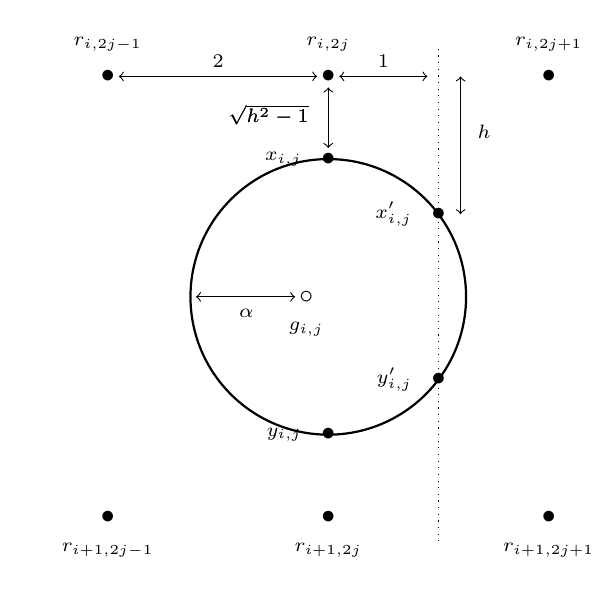
\begin{tikzpicture}[scale=7]

	
	\node[label=90:\scriptsize $r_{i,2j-1}$] at (0.1,0) {$\bullet$};
	\node[label=90:\scriptsize $r_{i,2j}$] at (0.5,0) {$\bullet$};
	\node[label=90:\scriptsize $r_{i,2j+1}$] at (0.9,0) {$\bullet$};
	
	\node[label=180:\scriptsize $\sqrt{h^2-1}$] at (0.5,-0.07) {};
	\node[label=180:\scriptsize $x_{i,j}$] at (0.5,-0.15) {$\bullet$};
	
	
	\node[label=180:\scriptsize $h$] at (0.83,-0.1) {};
	\node[label=180:\scriptsize $x_{i,j}'$] at (0.7,-0.25) {$\bullet$};
	
	\node[label=270:\scriptsize $g_{i,j}$] at (0.46,-0.4) {$\circ$};
	
	
	\node[label=180:\scriptsize $y_{i,j}$] at (0.5,-0.65) {$\bullet$};
	\node[label=180:\scriptsize $y_{i,j}'$] at (0.7,-0.55) {$\bullet$};
	
	
	\node[label=270:\scriptsize $r_{i+1,2j-1}$] at (0.1,-0.8) {$\bullet$};
	\node[label=270:\scriptsize $r_{i+1,2j}$] at (0.5,-0.8) {$\bullet$};
	\node[label=270:\scriptsize $r_{i+1,2j+1}$] at (0.9,-0.8) {$\bullet$};
	
	
	\node[label=180:\scriptsize $\sqrt{h^2-1}$] at (0.5,-0.07) {};
	
	
	\node[label=180:\scriptsize $\alpha$] at (0.4,-0.43) {};
	\node[label=90:\scriptsize $1$] at (0.6,-0.02) {};
	\node[label=90:\scriptsize $2$] at (0.3,-0.02) {};
	
	
	\draw[<->] (0.5,-0.13) -- (0.5,-0.02);
	\draw[<->] (0.26,-0.4) -- (0.44,-0.4);
	\draw[dotted,-] (0.7, 0.05) -- (0.7, -0.85);
	\draw[<->] (0.74, 0.0) -- (0.74, -0.25);
	\draw[<->] (0.68, 0.0) -- (0.52, 0.0);
	\draw[<->] (0.12, 0.0) -- (0.48, 0.0);
	\draw[black, thick] (0.5,-0.4) circle (0.25);
\end{tikzpicture}


\ifdefined\COMPLETE
\else
\end{document}
\fi

    \caption{The locations of $x_{i,j}$, $x_{i,j}'$, $y_{i,j}$ and $y_{i,j}'$ in the set $Z_i$. Note that the point $g_{i,j}$ is not vertically aligned with $x_{i, j}$ or $r_{i, 2j}$. This figure is adapted from \cite{vattani2009hardness}.}
    \label{fig:ZFig}
  \end{minipage}
\end{figure}


\begin{lemma}
\label{lemma:kmeansEquivalenceX3C}
The set $X = H_{l,n} \cup Z$ has a $k$-clustering of cost less or equal to $L$ if and only if there is an exact cover for the X3C instance.
\end{lemma}

\begin{lemma}
\label{lemma:gammaLower}
Any $k$-clustering of $X = H_{l,n} \cup Z$ with cost $\le L$ has the $\gamma$-margin property where $\gamma = \sqrt{3.4}$. Furthermore, $k = \Theta(n^{\epsilon})$.
\end{lemma}

The proofs are provided in Appendix \ref{appendix:lowerBoundProof}. Lemmas \ref{lemma:kmeansEquivalenceX3C} and \ref{lemma:gammaLower} together show that $X$ has a $k$-clustering of cost $\le L$ satisfying the $\gamma$-margin property (for $\gamma = \sqrt{3.4}$) if and only if there is an exact cover by $3$-sets for the X3C instance. This completes the proof of our main result (Thm. \ref{thm:gammaLower}). 

\subsection{Lower Bound on the Number of Queries}
In the previous section we showed that $k$-means clustering is NP-hard for $\gamma < \sqrt{3.4} \approx 1.84$ if the algorithm doesn't have access to any queries. On the other hand, if the algorithm has access to $O(k\log n)$ queries then the same problem ($k$-means clustering under $\gamma$-margin is easy. The following question arises. ``What happens if the algorithm has access to $o(k\log n)$ queries?" The theorem below shows that if the number of queries is $O(\log n)$ then the problem still remains NP-Hard.

\begin{theorem}
\label{thm:queryLower}
For any $\gamma \le \sqrt{3.4}$, finding the optimal solution to the $k$-means objective function is NP-Hard even when the optimal clustering satisfies the $\gamma$-margin property and the algorithm can ask $O(\log k + \log |\mc X|)$ same-cluster queries.
\end{theorem}

\begin{proof}
Proof by contradiction: assume that there is polynomial-time algorithm $\mc A$ that makes $O(\log k + \log |\mc X|)$ same-cluster queries to the oracle. Then, we show there exists another algorithm $\mc A^\prime$ for the same problem that is still polynomial but uses no queries. However, this will be a contradiction to Theorem \ref{thm:gammaLower}, which will prove the result.

In order to prove that such $\mc A^\prime$ exists, we use a `simulation' technique. Note that $\mc A$ makes only $q<\beta(\log k + \log |\mc X|)$ binary queries, where $\beta$ is a constant. The oracle therefore can respond to these queries in maximum $2^{q} < k^\beta|\mc X|^\beta$ different ways. Now the algorithm $\mc A^\prime$ can try to simulate all of $k^\beta|\mc X|^\beta$ possible responses by the oracle and output the solution with minimum $k$-means clustering cost. Therefore, $\mc A^\prime$ runs in polynomial-time and is equivalent to $\mc A$.
\end{proof}










%======================================================================
\chapter{Conclusion and Future Work}
\label{FUTURE}
%======================================================================
\section{Dealing with computational complexity}
We have discussed the computational challenges in clustering. The way around this is to show that clustering is easy when the data has certain nice properties (or clusterable). Various notions of clusterability have been proposed in the literature. Any notion of clusterability must satisfy the following requirements \cite{ben2015computational}. 

\begin{enumerate}
\item \emph{Realistic}

A lot the datasets in practice that we wish to cluster should satisfy this assumption. If a generative model is available, then data generated from that model should satisfy the clusterability assumption with high probability. Most of the notions in literature don't satisfy any of these conditions.

For our notion of sparse noise, we do provide some justification when the noise is generated by a non-concentrated distribution (Chapter \ref{ANALYSIS}). Our definition is much less restrictive than previous definitions and `seems' to be realistic. However, to truly satisfy this criteria, we need to answer the following question. 
\begin{itemize}
\item Can we find atleast a few datasets that satisfy our criteria?
\item Can we find some generative models which generate data satisfying sparse noise condition?
\end{itemize}

\item \emph{Efficient algorithms}

Another important requirement is that if the data is clusterable then there should exist efficient algorithms which find that clustering. For our notion of sparse noise, we proposed an algorithm which finds efficient representation of all nice solutions (Chapter \ref{ANALYSIS}). We also give conditions under which finding all solutions is not possible. However, some questions still remain unanswered. \begin{itemize}
\item What if the goal is to find only one such nice solution and not to represent all nice solutions?
\item Is it possible to propose a clustering objective which finds the nice solution if the data is clusterable? 
\end{itemize}

\item \emph{Verification}
\begin{itemize}
\item Given any dataset, is there an algorithm which answers yes or no depending upon whether the dataset satisfies our clusterability notion? 
\end{itemize}
So far, we and any of the previous works have not addressed this question in great detail.

\item \emph{Performance of popular algorithms }(not essential)
\begin{itemize}
\item Can we show that popular algorithms like $k$-means or $k$-median are guaranteed to converge to an optimal or near-optimal solution if the data satisfies our clusterability notion? 
\end{itemize}
Ben-David et. al \cite{ben2014clustering} and Ostrovsky et. al \cite{ostrovsky2006effectiveness} try to address this issue but they impose very strong assumptions on the data. Hence, they end up violating the first principle that the notion should be realistic. Another reason why it might be difficult to prove convergence for $k$-means or $k$-median is that they are sensitive to even one single point. The following question which is similar to Q2.2 is interesting.
\begin{itemize}
\item Is it possible to propose a clustering objective which handles noisy points?
\end{itemize}

\end{enumerate}


\section{Dealing with under-specificity}
We have discussed that under-specificity due to the existence of multiple `correct' solutions is a major challenge in clustering. To tackle this challenge, we need to incorporate domain-expertise into clustering. This can be done by introducing human supervision into the clustering problem. Any framework of semi-supervised clustering should satisfy the following properties.

\begin{enumerate}
\item \emph{Realistic}

The form of supervision suggested should be implementable in practice. In one of the models, supervision is provided by the expert clustering a small subset. If supervision is provided by answering queries then it should be reasonable to assume that a user (or an expert) can answer such queries. For example, in the merge-split model of Balcan et. al \cite{balcan2008clustering} can a user be expected to evaluate a clustering of a big dataset and then suggest which clusters to merge/split? Our model of same-cluster query seems realistic. However, to truly satisfy this criteria, we need to answer the following question. 
\begin{itemize}
\item Can we find atleast a few datasets that satisfy our criteria?
\end{itemize}
In a realistic setting, it is possible that a user may not be able to answer a few queries or maybe even make an error in some of the cases.
\begin{itemize}
\item Can we extend our framework to handle user mistakes? 
\item Can we extend our framework to handle user abstensions?
\item Can we extend our framework to handle noisy points where there is no clear cluster membership? 
\end{itemize}

\item \emph{Efficient algorithms}

Another important requirement is that using only \textbf{weak} supervision (for example using only a small number of queries) our algorithm should converge to the true clustering. Querying the oracle is an expensive operation. Our current algorithm makes $O(k\log n + k^2\log k)$ queries. 
\begin{itemize}
\item Can we improve the number of queries while relaxing some of the other parameters like data niceness etc.?
\end{itemize}
Another approach to deal with under-specificity is to allow an algorithm to output multiple solutions. 
\begin{itemize}
\item Given a hierarchical clustering tree or a small list of clusterings, is it possible to find the true clustering by making fewer queries?
\end{itemize}

\end{enumerate}







%=============================================================================


\appendix
\chapter{Comparison of $\gamma$-Margin and $\alpha$-Center Proximity}
\section{Centers from data}
\begin{theorem}
\label{thm:upperCenterData}
Let $(X , d)$ be a clustering instance and $\gamma \ge 2$. Then, Algorithm 1 in \cite{balcan2012clustering} outputs a tree $\mc T$ with the following property: 


Any $k$-clustering $\mc C^* = \{C_1^*, \ldots, C_k^* \}$ which satisfies the $\gamma$-margin property and its cluster centers $\mu_1, \ldots, \mu_k$ are in $X$, is a pruning of the tree $T$. In other words, for every $1 \le i \le k$, there exists a node $N_i$ in the tree $T$ such that $C_i^* = N_i$.
\end{theorem}

\begin{proof}
Let $p, p' \in C_i^*$ and $q \in C_j^*$. \cite{balcan2012clustering} prove the correctness of their algorithm for $\alpha > \sqrt{2} + 1$. Their proof relies only on the following three properties which are implied when $\alpha > \sqrt{2} + 1$. We will show that these properties are implied by $\gamma > 2$ instances as well.
\begin{itemize}
\item $d(p, \mu_i) < d(p, q)$\\
$\gamma d(p, \mu_i) < d(q, \mu_i) < d(p, q) + d(p, \mu_i) \implies d(p, \mu_i) < \frac{1}{\gamma-1}d(p, q)$.
\item $d(p, \mu_i) < d(q, \mu_i)$\\
This is trivially true since $\gamma > 2$.
\item $d(p, \mu_i) < d(p', q)$\\
Let $r = \max_{x \in C_i^*} d(x, \mu_i)$. Observe that $d(p, \mu_i) < r$. Also, $d(p', q)> d(q, \mu_i)-d(p', \mu_i) > \gamma r - r = (\gamma -1)r$.
\end{itemize}
\end{proof}

\begin{theorem}
\label{thm:lowerCenterData}
Let $(\mc X, d)$ be a clustering instance and $k$ be the number of clusters. For $\gamma < 2$, finding a $k$-clustering of $X$ which satisfies the $\gamma$-margin property and where the corresponding centers $\mu_1, \ldots, \mu_k$ belong to $\mc X$ is NP-Hard.
\end{theorem}
\begin{proof}
For $\alpha < 2$, \cite{ben2014data} proved that in general metric spaces, finding a clustering which satisfies the $\alpha$-center proximity and where the centers $\mu_1, \ldots, \mu_k \in \mc X$ is NP-Hard. Note that the reduced instance in their proof, also satisfies $\gamma$-margin for $\gamma < 2$. 
\end{proof}

\section{Centers from metric space}
\begin{theorem}
\label{thm:upperCenterMetric}
Let $(X , d)$ be a clustering instance and $\gamma \ge 3$. Then, the standard single-linkage algorithm outputs a tree $\mc T$ with the following property:


Any $k$-clustering $\mc C^* = \{C_1^*, \ldots, C_k^* \}$ which satisfies the $\gamma$-margin property is a pruning of $T$. In other words, for every $1 \le i \le k$, there exists a node $N_i$ in the tree $T$ such that $C_i^* = N_i$. 
\end{theorem}

\begin{proof}
\cite{balcan2008discriminative} showed that if a clustering $C^*$ has the strong stability property, then single-linkage outputs a tree with the required property. It is simple to see that if $\gamma > 3$ then instances have strong-stability and the claim follows.  
\end{proof}


\begin{theorem}
\label{thm:lowerCenterMetric}
Let $(\mc X, d)$ be a clustering instance and $\gamma < 3$. Then, finding a $k$-clustering of $X$ which satisfies the $\gamma$-margin is NP-Hard.
\end{theorem}
\begin{proof}
\cite{awasthi2012center} proved the above claim but for $\alpha < 3$ instances. Note however that the construction in their proof satisfies $\gamma$-margin for $\gamma < 3$. 
\end{proof}








\chapter{Proofs of missing lemmas and theorems from Chapter \ref{ANALYSIS}}
\textbf{Proof of Theorem~\ref{thm:alphacpnoise}}
Fix any $\mc S \subseteq \mc X$. Let $\mc C^*_S = \{S_1^*, \ldots, S_k^*\}$ be a clustering of $\mc S$ such that $m(\mc C_{\mc S}^*) = t$ and $\mc C^*_S$ has $(\alpha, \eta)$-center proximity. Denote by $r_i := r(S_i^*)$ and $r = \max r_i$. Define $Y_B^{\mc C} := \{C_i \in \mc C : C_i \subseteq B \text{ or } |B \cap C_i| \ge t/2\}$. Note that whenever a ball $B$ satisfies the sparse-distance condition, all the clusters in $Y_{B}^{{\mc C}^{(l)}}$ are merged together and the clustering $\mc C^{(l+1)}$ is updated. We will prove the theorem by proving two key facts.

\begin{enumerate}[label=\textbf{F.\arabic*},leftmargin=0.3in]
\renewcommand\labelitemi{$\diamond$}
\item \label{fact:1} If the algorithm merges points from a good cluster $S_i^*$ with points from some other good cluster,  then at this step the distance being considered $d = d(p,q) > r_i$.	
\item \label{fact:2} When the algorithm considers the distance $d = r_i$, it merges all points from $S_i^*$ (and possibly points from $\mc X\setminus \mc S$) into a single cluster $C_i$. Hence, there exists a node in the tree $N_i$ which contains all the points from $S_i^*$ and no points from any other good cluster $S_j^*$. 	
\end{enumerate}
Note that the theorem follows from these two facts. Similar reasoning was also used in proof of Lemma 3 in \cite{balcan2012clustering}. We now prove both of these facts formally. 

\noindent\textit{\underline{Proof of Fact.~\ref{fact:1}}}
Let $\mc C^{(l)} = \{C_1, \ldots, C_{k'}\}$ be the current clustering of $\mc X$. Let $l+1$ be the first merge step which merges points from the good cluster $S_i^*$ with points from some other good cluster. Let $p, q \in \mc X$ be the pair of points being considered at this step and $B = B(p, d(p, q))$ the ball that satisfies the sparse distance condition at this merge step. Denote by $Y = Y_{B}^{C^{(l)}}$. We need to show that $d(p, q) > r_i$. To prove this, we need Claim~\ref{claim:fromBothCluster} below. 

\begin{smallLemma}
\label{claim:fromBothCluster}
Let $p, q \in \mc X$ and $B$, $Y$, $S_i^*$ and $C^{(l)}$ be as defined above. If $d(p, q) \le r,$ then $B \cap S_i^* \neq \emptyset$ and there exists $n \neq i$ such that $B \cap S_n^* \neq \emptyset$.
\end{smallLemma}
\vspace{-0.1in} $l+1$ is the first step which merges points from $S_i^*$ with some other good cluster. Hence, $\exists C_i \in Y$ such that $C_i\cap S_i^*  \neq \emptyset$ and $\forall n \neq i$, $C_i \cap S_n^* = \emptyset$. Also, $\exists C_j \in Y$ such that $C_j \cap S_j^* \neq \emptyset$ for some $S_j^*$ and $C_j \cap S_i^* = \emptyset$.

$C_i \in Y$. Hence, $C_i \subseteq B$ or $|C_i \cap B| \ge t/2$. The former is trivial. In the latter, for the sake of contradiction, assume that $B$ contains no points from $S_i^*$. This implies that $B \cap C_i \subseteq B \cap \{\mc X \setminus \mc S\}$ and $|B\cap \{\mc X \setminus \mc S\}| \ge t/2$. This  is a contradiction. The case when $C_j \in Y$ is identical. \qed

\begin{smallLemma}
\label{claim:maxrirj}
Let the framework be as given in Claim~\ref{claim:fromBothCluster}. Then, $d(p, q) > r_i$.
\end{smallLemma}

\vspace{-0.1in} \noindent If $d(p, q) > r$, then the claim follows trivially. In the other case, from Claim~\ref{claim:fromBothCluster}, $B$ contains $p_i \in S_i^*$ and $p_j \in S_j^*$. Let $r_i = d(c_i, q_i)$ for some $q_i \in S_i^*$.

$d(c_i, q_i) < \frac{1}{\alpha} d(q_i, c_j) < \frac{1}{\alpha} [ \frac{1}{\alpha}d(p_i, p_j) + \frac{1}{\alpha}d(c_i, q_i) + d(p_i, p_j) + 2d(c_i, q_i)]$
This implies that $(\alpha^2 - 2\alpha - 1)d(q_i, c_i) < (\alpha + 1) d(p_i, p_j)$. For $\alpha \ge 2 + \sqrt 7$, this implies that $d(c_i, q_i) < d(p_i, p_j)/2$ which implies $d(c_i, q_i) < d(p, q)$. This result was also stated in \cite{balcan2012clustering}.\qed

\noindent\textit{\underline{Proof of Fact \ref{fact:2}
}}
Let $\mc C^{(l)} = \{C_1, \ldots, C_{k'}\}$ be the current clustering of $\mc X$. Let $l+1$ be the merge step when $p = s_i$ and $q = q_i$ such that $d(s_i, q_i) = r_i$. We will prove that the ball $B = B(s_i, q_i)$ satisfies the sparse-distance condition.

\begin{smallLemma}
%\vspace{-0.1in}
\label{claim:dciqi}
Let $s_i$, $q_i$, $r_i$, $B$ and $Y$ be as defined above. Then, $B$ satisfies the sparse distance condition and for all $C \in Y$, for all $j \neq i, C \cap S_j^* = \emptyset$.
\end{smallLemma}
\vspace{-0.1in} $|B| = |S_i^*| \ge t$. Observe that, for all $C \in \mc C^{(l)}$, $|C| = 1$ or $|C| \ge t$. 

\begin{itemize}[nolistsep,leftmargin=*]
\item Case 1. $|C| = 1$. If $C \cap B \neq \emptyset \implies C \subseteq B = S_i^*$.
\item Case 2. $|C|\ge t$. $C \cap B \neq \emptyset$. Let $h(C)$ denote the height of the cluster in the tree $T$. 
\begin{itemize}[leftmargin=*]
\renewcommand\labelitemii{$\circ$}
\item Case 2.1. $h(C) = 1$. In this case, there exists a ball $B'$ such that $B' = C$. We know that $r(B') \le r_i \le r$. Hence using Claim~\ref{claim:maxrirj}, we get that for all $j \neq i$, $B' \cap S_j^* = \emptyset$. Thus, $|B'\setminus S_i^*| \le t/2 \implies |B\cap C| = |C| - |C\setminus B| = |C| - |B'\setminus S_i^*| \ge t/2$. Hence, $C \in Y$.

\item Case 2.2. $h(C) > 1$. Then there exists some $C'$ such that $h(C') = 1$ and $C' \subset C$. Now, using set inclusion and the result from the first case, we get that $|B\cap C| \ge |B\cap C'| \ge t/2$. Hence, $C \in Y$. Using Claim~\ref{claim:maxrirj}, we get that for all $j \neq i$, $C \cap S_j^* = \emptyset$.\qed\\
\end{itemize} 
\end{itemize}


\noindent\textbf{Proof of Theorem~\ref{thm:noalgalphacp}}
Let $\mc X, B_1, B_2, B_1', B_2'$ be as shown in Fig. \ref{fig:noalgalphacp}. Let $t_1 = \frac{t}{2}+1$ and $t_2 = \frac{t}{2}-2$. For $\alpha \le 2+\sqrt{3}$, clusterings $\mc C_{\mc S} = \{B_1, B_2, B_3, \ldots, B_k\}$ and $\mc C_{\mc S'} = \{\ B_1', B_2', B_3, \ldots, B_k\}$ satisfy $(\alpha, 1)$-center proximity and $m(\mc C_{\mc S}) = m(\mc C_{\mc S}') = t$. Now, a simple proof by contradiction shows that there doesn't exist a tree $T$ and prunings $P$ and $P'$ such that $P$ respects $\mc C_{\mc S}$ and $P'$ respects $\mc C_{\mc S'}$. \qed\\

\begin{figure}[!t]
\begin{center}
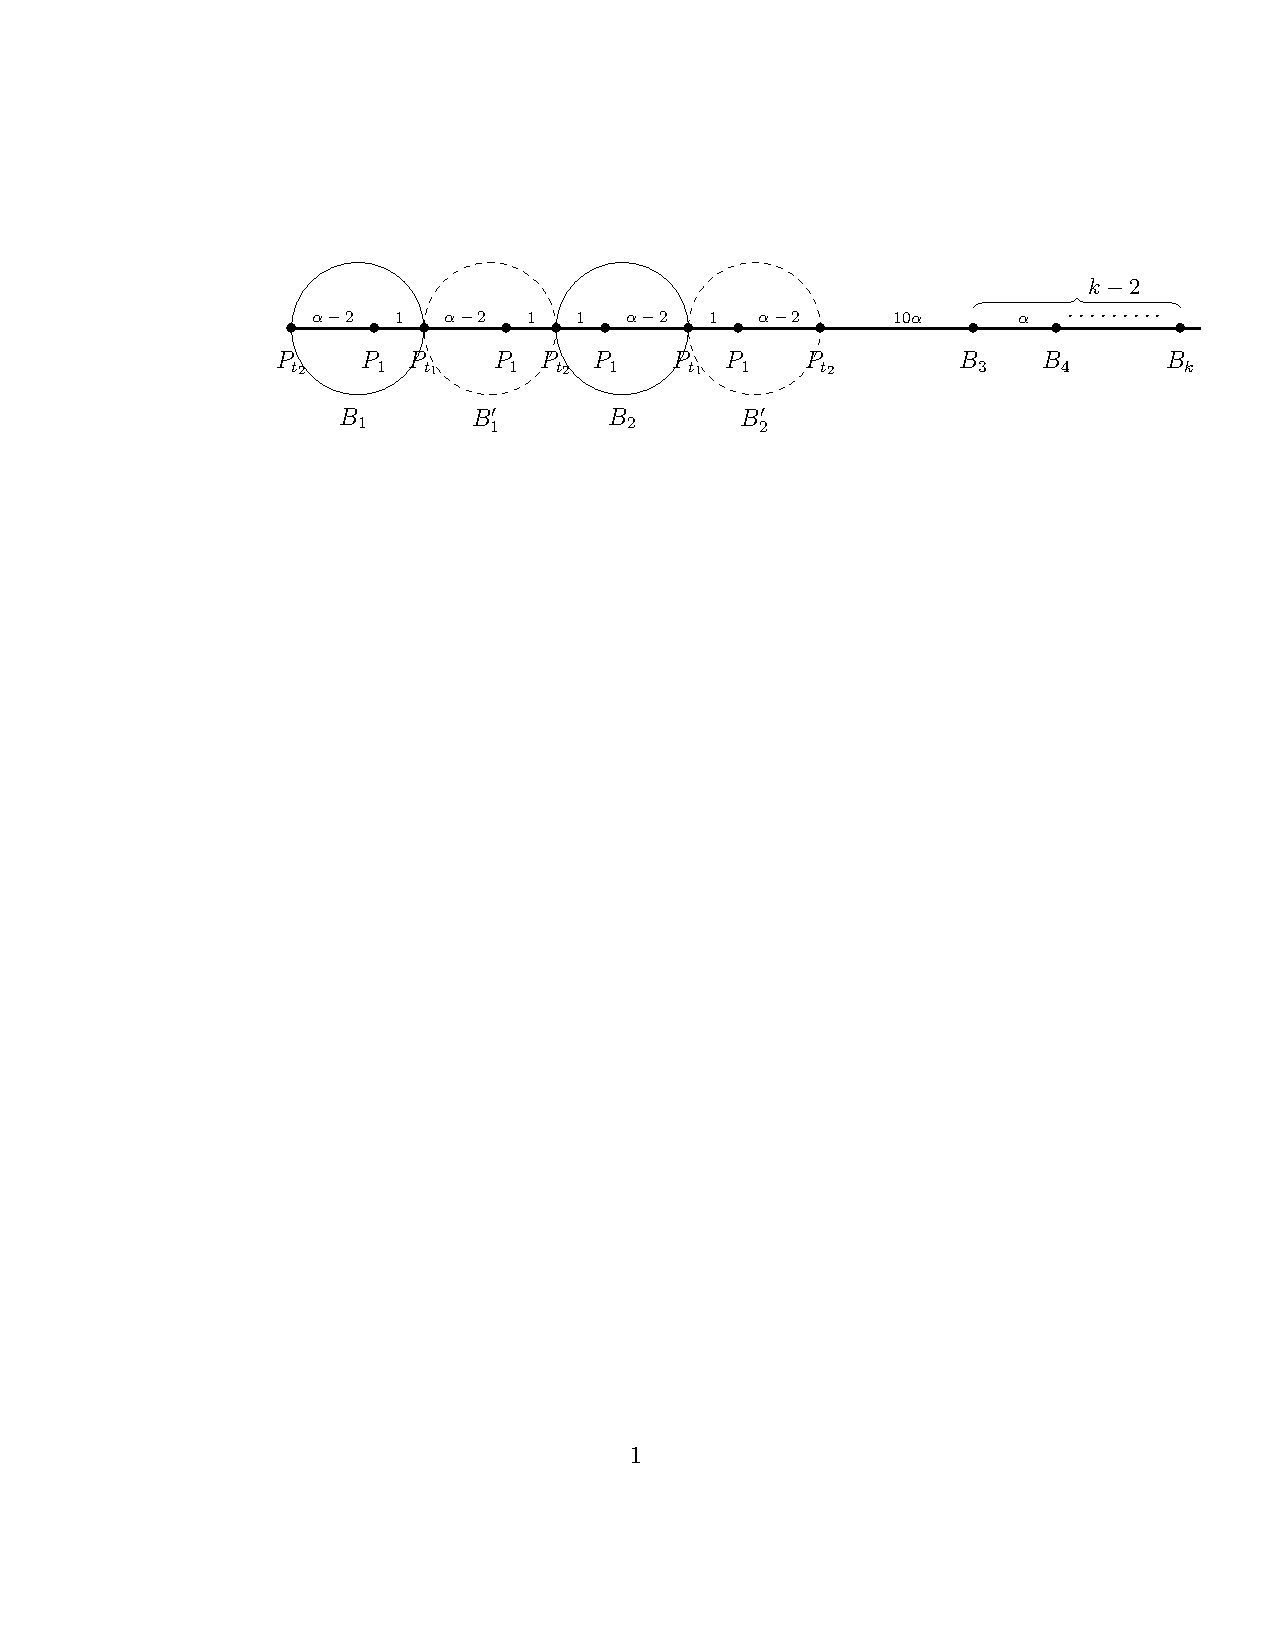
\includegraphics[trim={47mm 205mm 12mm 44mm},clip,width=\textwidth]{figures/lbdFig2.pdf}
\end{center}
\caption{$\mc X \subseteq \mathbb{R}$ such that no tree can capture all the $(\alpha, \eta)$-proximal clusterings.}
\label{fig:noalgalphacp}
\end{figure}

\noindent\textbf{Proof of Theorem~\ref{thm:nolistalphacp}}
The clustering instance $\mc X$ is an extension of Fig. \ref{fig:noalgalphacp}. Let  \\$G_1 = \{B_1, B_1', B_2, B_2'\}$ be the balls as in Fig. \ref{fig:noalgalphacp}. Now, construct $G_2 = \{B_3, B_3', B_4, B_4'\}$ exactly identical to $G_1$ but far. In this way, we construct $k/2$ copies of $G_1$. \qed\\

\noindent\textbf{Proof of Theorem~\ref{thm:nosparsealg}}
Let $\mc X \subseteq \mathbb{R}$ be as shown in Fig. \ref{fig:nosparsealg}. Let $t' = \frac{t}{2}-1$ and let $B_1, B_2, B_3, B_1'$, $B_2', B_3', B_1'', B_2''$ and $B_3''$ be as shown in Fig.~\ref{fig:nosparsealg}. For $\alpha \le 2\sqrt{2}+3$, clusterings \\$\mc C_{\mc S} = \{B_1, B_2, B_3, \ldots, B_k\}$, $\mc C_{\mc S'} = \{\ B_1', B_2', B_3, \ldots, B_k\}$ and $\mc C_{\mc S}'' = \{\ B_1'', B_2'', B_3, \ldots, B_k\}$ satisfy $(\alpha, 1)$-center proximity. Also, $m(\mc C_{\mc S}) = m(\mc C_{\mc S}') =$ $m(\mc C_{\mc S}'') = t$. Arguing similarly as in Theorem \ref{thm:noalgalphacp} completes the proof. \qed\\
\begin{figure}[!t]
\begin{center}
\includegraphics[trim={45mm 210mm 20mm 43mm},clip,width=\textwidth]{figures/lbdFig3.pdf}
\end{center}
\caption{$\mc X \subseteq \mathbb{R}$ such that no algorithm can capture all the $\alpha$-proximal clusterings. } 
\label{fig:nosparsealg}
\end{figure}

\noindent\textbf{Proofs of Theorems~\ref{thm:nosparselistalphacp}, \ref{thm:nosparselistlambdacs} and \ref{thm:nolistlambdacs}} have the exact same ideas as the proof of Theorem~\ref{thm:nolistalphacp}. To prove the lower bound in the list model, instance constructed in Theorem~\ref{thm:nolistalphacp} is a simple extension of the instance in Theorem~\ref{thm:noalgalphacp}. The instances for the proof of Theorems~\ref{thm:nosparselistalphacp}, \ref{thm:nosparselistlambdacs} and \ref{thm:nolistlambdacs} are similarly constructed as extensions of their respective tree lower bound instances (Theorems~\ref{thm:nosparsealg}, \ref{thm:nosparselambdaalg} and \ref{thm:noalglambdacs}).

\noindent\textbf{Proof of Theorems~\ref{thm:nosparselambdaalg} and \ref{thm:noalglambdacs}} are also identical to the proofs of Theorem~\ref{thm:nosparsealg} and \ref{thm:noalgalphacp}.\\

\noindent\textbf{Proof of Theorem~\ref{thm:lambdacsnoise}}
Fix $\mc S \subseteq \mc X$. Denote by $r_i := r(S_i^*)$. Let $\mc C_{\mc X} = \{C_1, \ldots, C_k\}$ be the clustering outputed by the algorithm. Let $\mc L = \{B_1, \ldots, B_l\}$ be the list of balls as outputed by Phase 1 of Alg.~\ref{alg:lambdacs}. Let $G$ be the graph as constructed in Phase 2 of the algorithm. Observe that $B = B(s_i, r_i) = S_i^* \in \mc L$. WLOG, denote this ball by $B^{(i)}$ and the corresponding vertex in the graph $G$ by $v^{(i)}$. We will prove the theorem by proving two key facts.  

\begin{enumerate}[nolistsep,noitemsep,label=\textbf{F.\arabic*},leftmargin=0.3in]
\renewcommand\labelitemi{$\diamond$}
\item \label{fact:lambda1} If $B_{i1}$ and $B_{i2}$ intersect $S_i^*$ then the vertices $v_{i1}$ and $v_{i2}$ are connected.
\item \label{fact:lambda2} If $B_{i1}$ intersects $S_i^*$ and $B_{j1}$ intersects $S_j^*$ then $v_{i1}$ and $v_{j1}$ are disconnected in $G$.	
\end{enumerate}

\vspace{-0.1in}
\begin{smallLemma}
\label{claim:lambda1}
Let $\mc L, G, B^{(i)}$ and $v^{(i)}$ be as defined above. Let balls $B_{i1}, B_{i2} \in \mc L$ be such that $B_{i1} \cap S_i^* \neq \emptyset$ and $B_{i2} \cap S_i^* \neq \emptyset$. Then there exists a path between $v_{i1}$ and $v_{i2}$.
\end{smallLemma}
\vspace{-0.1in} Assume that $v_{i1}$ and $v^{(i)}$ are not connected by an edge. Hence, $|B_{i1} \setminus B^{(i)}| \ge t/2$. Since $\lambda > 4$, for all $j \neq i$, $B_{i1} \cap S_j^* = \emptyset$. Thus, $B_{i1} \setminus B^{(i)} \subseteq \mc X \setminus \mc S$. which contradicts $|B_{i1} \cap \{\mc X \setminus \mc S\}| < t/2$.\qed

%\vspace{-0.1in}
\begin{smallLemma}
Let the framework be as in Claim~\ref{claim:lambda1}. Let $B_{i1} \in \mc L$ be such that $B_{i1} \cap S_i^* \neq \emptyset$ and $B_{j1}$ be such that $B_{j1} \cap S_j^* \neq \emptyset$. Then $v_{i1}$ and $v_{j1}$ are disconnected in $G$.
\end{smallLemma}
\vspace{-0.1in} Assume that $v_{i1}$ and $v_{j1}$ are connected. Hence, there exists vertices $v_{i}$ and $v_{n}$ such that $v_i$ and $v_n$ are connected by an edge in $G$ and $B_i \cap S_i^* \neq \emptyset$ and $B_n \cap S_n^* \neq \emptyset$ for some $n \neq i$. $|B_i \cap B_n| \ge t/2$. Now, $\lambda \ge 4$, thus $B_i \cap \{\mc S \setminus S_i^*\} = \emptyset$ and $B_n \cap \{\mc S\setminus S_n^*\} = \emptyset$. Thus, $B_i \cap B_n \subseteq \mc X \setminus \mc S$ which contradicts the sparseness assumption.
\qed

\label{appendix:sectiontr}
\begin{theorem}[Vapnik and Chervonenkis \cite{vapnik2015uniform}]\label{theorem:vceapprox}
Let $X$ be a domain set and $D$ a probability distribution over $X$. Let $H$ be a class of subsets of $X$ of finite VC-dimension $d$. Let $\epsilon, \delta \in (0,1)$. Let $S \subseteq X$ be picked i.i.d according to $D$ of size $m$. If $m > \frac{c}{\epsilon^2}(d\log \frac{d}{\epsilon}+\log\frac{1}{\delta})$, then  with probability $1-\delta$ over the choice of $S$, we have that $\forall h \in H$
$$\bigg|\frac{|h\cap S|}{|S|} - P(h)\bigg| < \epsilon$$
\end{theorem}







\chapter{Proofs of missing lemmas and theorems from Chapter \ref{SSC}}
\label{appendix:lowerBoundProof}

In Section \ref{section:lowerBounds} we proved Theorem \ref{thm:gammaLower} based on two technical results (i.e., lemma \ref{lemma:kmeansEquivalenceX3C} and \ref{lemma:gammaLower}). In this appendix we provide the proofs for these lemmas. In order to start, we first need to establish some properties about the Euclidean embedding of $X$ proposed in Section \ref{section:lowerBounds}.

%$$L_1 = (6m+3)w, L_2 = 6m(l-1), L=L_1 + L_2, \alpha = \frac{d}{w}-\frac{1}{2w^3}$$

\begin{definition}[$A$- and $B$-Clustering of $R_i$]
\label{defn:abclusteringVattani}

An $A$-Clustering of row $R_i$ is a clustering in the form of $\{\{s_i\}, \{r_{i,1}, r_{i,2}\}, \{r_{i,3}, r_{i,4}\}, \ldots,$ $ \{r_{i,6m-1}, r_{i,6m}\},\{r_{i, 6m+1}, f_i\}\}$. A $B$-Clustering of row $R_i$ is a clustering in the form of $\{\{s_i, r_{i, 1}\}, \{r_{i,2}, r_{i,3}\}, \{r_{i,4}, r_{i,5}\}, \ldots,$ $ \{r_{i,6m}, r_{i,6m+1}\},\{f_i\}\}$. 
\end{definition}

\begin{definition}[Good point for a cluster]
\label{defn:goodPointVattani}
A cluster $C$ is good for a point $z \not\in C$ if adding $z$ to $C$ increases cost by exactly $\frac{2w}{3}h^2$ 
\end{definition}

Given the above definition, the following simple observations can be made. 
\begin{itemize}[nolistsep,noitemsep]
\item The clusters $\{r_{i,2j-1}, r_{i, 2j}\}$, $\{r_{i,2j}, r_{i, 2j+1}\}$ and $\{g_{i,j}\}$ are good for $x_{i,j}$ and $y_{i-1,j}$.
\item The clusters $\{r_{i,2j}, r_{i, 2j+1}\}$ and $\{g_{i,j}\}$ are good for $x_{i,j}'$ and $y_{i-1,j}'$.
\end{itemize}

\begin{definition}[Nice Clustering]
\label{defn:niceClustering}
A $k$-clusteirng is nice if every $g_{i,j}$ is a singleton cluster, each $R_i$ is grouped in the form of either an $A$-clustering or a $B$-clustering, and each point in $Z_i$ is added to a cluster which is good for it.
\end{definition}

It is straightforward to see that a row grouped in a $A$-clustering costs $(6m+3)w-\alpha$ while a row in $B$-clustering costs $(6m+3)w$. Hence, a nice clustering of $H_{l,m} \cup Z$ costs at most $L_1 + L_2$. More specifically, if $t$ rows are group in a $A$-clustering, the nice-clustering costs $L_1+L_2-t\alpha$. Also, observe that any nice clustering of $X$ has only the following four different types of clusters. \begin{enumerate}[label=(\arabic*),nolistsep,leftmargin=*]
\item Type E - $\{r_{i,2j-1}, r_{i,2j+1}\}$ \\
The cost of this cluster is $2w$ and the contribution of each location to the cost (i.e., $\frac{cost}{\#locations}$) is $ \frac{2w}{2} = w$.
\item Type F - $\{r_{i,2j-1}, r_{i, 2j}, x_{i, j}\}$ or $\{r_{i,2j-1}, r_{i, 2j}, y_{i-1, j}\}$ or $\{r_{i,2j}, r_{i, 2j+1}, x_{i, j}'\}$ or $\{r_{i,2j}, r_{i, 2j+1}, y_{i-1, j}'\}$\\
The cost of any cluster of this type is $2w(1+\frac{h^2}{3})$ and the contribution of each location to the cost is at most $\frac{2w}{9}(h^2+3)$. This is equal to $\frac{16}{9}w$ because we had set $h = \sqrt 5$.
\item Type I - $\{g_{i, j}, x_{i,j}\}$ or $\{g_{i, j}, x_{i,j}'\}$  or $\{g_{i, j}, y_{i,j}\}$  or $\{g_{i, j}, y_{i,j}'\}$\\
The cost of any cluster of this type is $\frac{2}{3}wh^2$ and the contribution to the cost of each location is $\frac{w}{3}h^2$. For our choice of $h$, the contribution is $\frac{5}{3}w$.
\item Type J - $\{s_i, r_{i,1}\}$ or $\{r_{i,6m+1}, f_i\}$\\
The cost of this cluster is $3w$ (or $3w-\alpha$) and the contribution of each location to the cost is at most $1.5w$. 
\end{enumerate}
Hence, observe that in a nice-clustering, any location contributes at most $\le \frac{16}{9}w$ to the total clustering cost. This observation will be useful in the proof of the lemma below.

\begin{lemma}
\label{lemma:costNonNice}
For large enough $w = poly(l, m)$, any non-nice clustering of $X = H_{l, m} \cup Z$ costs at least $L + \frac{w}{3}$.
\end{lemma}

\begin{proof}
We will show that any non-nice clustering $C$ of $X$ costs at least $\frac{w}{3}$ more than any nice clustering. This will prove our result. The following cases are possible.

\begin{itemize}[nolistsep,leftmargin=*]
\item $C$ contains a cluster $C_i$ of cardinality $t > 6$ (i.e., contains $t$ weighted points)\\
Observe that any $x \in C_i$ has at least $t-5$ locations at a distance greater than 4 to it, and $4$ locations at a distance at least $2$ to it. Hence, the cost of $C_i$ is at least $\frac{w}{2t}(4^2(t-5)+2^24)t = 8w(t-4)$. $C_i$ allows us to use at most $t-2$ singletons. This is because a nice clustering of these $t+(t-2)$ points uses at most $t-1$ clusters and the clustering $C$ uses  $1 + (t-2)$ clusters for these points. The cost of the nice cluster on these points is $\le \frac{16w}{9}2(t-1)$. While the non-nice clustering costs at least $8w(t-4)$. For $t \ge 6.4 \implies 8(t-4) > \frac{32}{9}(t-1)$ and the claim follows. Note that in this case the difference in cost is at least $\frac{8w}{3}$. 

\item Contains a cluster of cardinality $t = 6$\\
Simple arguments show that amongst all clusters of cardinality $6$, the following has the minimum cost. $C_i = \{r_{i, 2j-1}, r_{i, 2j}, x_{i,j}, y_{i-1, j}, r_{i, 2j+1}, r_{2j+2}\}$. The cost of this cluster is $\frac{176w}{6}$. Arguing as before, this allows us to use $4$ singletons. Hence, a nice cluster on these $10$ points costs at most $\frac{160w}{9}$. The difference of cost is at least $34w$.  

\item Contains a cluster of cardinality $t = 5$\\
Simple arguments show that amongst all clusters of cardinality $5$, the following has the minimum cost. $C_i = \{r_{i, 2j-1}, r_{i, 2j}, x_{i,j}, y_{i-1, j}, r_{i, 2j+1}\}$. The cost of this cluster is $16w$. Arguing as before, this allows us to use $3$ singletons. Hence, a nice cluster on these $8$ points costs at most $16w\frac{8}{9}$. The difference of cost is at least $\frac{16w}{9}$.  

\item Contains a cluster of cardinality $t = 4$\\
It is easy to see that amongst all clusters of cardinality $4$, the following has the minimum cost. $C_i = \{r_{i, 2j-1}, r_{i, 2j}, x_{i,j}, r_{i, 2j+1}\}$. The cost of this cluster is $11w$. Arguing as before, this allows us to use $2$ singletons. Hence, a nice cluster on these $6$ points costs at most $\frac{32w}{3}$. The difference of cost is at least $\frac{w}{3}$.

\item All the clusters have cardinality $\le 3$ \\
Observe that amongst all non-nice clusters of cardinality $3$, the following has the minimum cost. $C_i = \{r_{i, 2j-1}, r_{i, 2j}, r_{i, 2j+1}\}$. The cost of this cluster is $8w$. Arguing as before, this allows us to use at most $1$ more singleton. Hence, a nice cluster on these $4$ points costs at most $\frac{64w}{9}$. The difference of cost is at least $\frac{8w}{9}$.

It is also simple to see that any non-nice clustering of size $2$ causes an increase in cost of at least $w$.

\end{itemize}
\end{proof}

%\begin{lemma}
%\label{lemma:kmeansEquivalenceX3C}
%The set $X = H_{l,n} \cup Z$ has a $k$-clustering %of cost less or equal to $L$ if and only if there %is an exact cover for the X3C instance.
%\end{lemma}
\begin{proof}[Proof of lemma \ref{lemma:kmeansEquivalenceX3C}]
The proof is identical to the proof of Lemma 11 in \cite{vattani2009hardness}. Note that the parameters that we use are different with those utilized by \cite{vattani2009hardness}; however, this is not an issue, because we can invoke our lemma \ref{lemma:costNonNice} instead of the analogous result in Vattani (i.e., lemma 10 in Vattani's paper). The sketch of the proof is that based on lemma \ref{lemma:costNonNice}, only nice clusterings of $X$ cost $\le L$. On the other hand, a nice clustering corresponds to an exact 3-set cover. Therefore, if there exists a clustering of $X$ of cost $\le L$, then there is an exact 3-set cover. The other way is simpler to proof; assume that there exists an exact 3-set cover. Then, the corresponding construction of $X$ makes sure that it will be clustered \emph{nicely}, and therefore will cost $\le L$.  



 %argue why the only nice clusterings of $X$ cost $\le L$. We use Lemma \ref{lemma:costNonNice} to argue the same. Note that since the parameters are much different that those considered in Vattani's original construction, we need to argue much more carefully to prove Lemma \ref{lemma:costNonNice}. 
\end{proof}

%\begin{lemma}
%\label{lemma:gammaLower}
%Any clustering of $X = H_{l,n} \cup Z$ which has %cost$\le L$ has the $\gamma$-margin property where %$\gamma = \sqrt{\frac{17}{5}} \approx 1.84$.
%\end{lemma}
\begin{proof}[Proof of lemma \ref{lemma:gammaLower}]
As argued before, any nice clustering has four different types of clusters. We will calculate the minimum ratio $a_i = \frac{d(y, \mu)}{d(x, \mu)}$ for each of these clusters $C_i$ (where $x \in C_i$, $y \not\in C_i$ and $\mu$ is mean of all the points in $C_i$.) Then, the minimum $a_i$ will give the desired $\gamma$. 
\begin{enumerate}[label=(\arabic*),nolistsep,leftmargin=*]
\item For Type E clusters $a_i = h/1 = \sqrt{5}$. 
\item For Type F clusters. $a_i = \frac{\frac{\sqrt{4+16(h^2-1)}}{3}}{2h/3} = \sqrt{\frac{17}{5}} \approx 1.84$. 
\item For Type I clusters, standard calculation show that $a_i > 2$.
\item For Type J clusters $a_i = \frac{2+\frac{\sqrt{6}}{2}}{\frac{\sqrt{6}}{2}} > 2$.
\end{enumerate}

\noindent Furthurmore, $|\mc X| = (12lm + 3l -6m)w$ and $k = 6lm + 2l - 3m$. Hence for $w = $poly$(l, m)$ our hardness result holds for $k = |\mc X|^{\epsilon}$ for any $0 < \epsilon < 1$.
\end{proof}
\noindent Lemmas \ref{lemma:kmeansEquivalenceX3C} and \ref{lemma:gammaLower} complete the proof of the main result (Thm. \ref{thm:gammaLower}). 


%================================================
%================================================
%================================================

\begin{theorem}[Generalized Hoeffding's Inequality (e.g., \cite{ashtiani2015dimension})]
\label{thm:genHoeff}
Let $X_1, \ldots. X_n$ be i.i.d random vectors in some Hilbert space such that for all $i$, $\|X_i\|_2 \le R$ and $E[X_i] = \mu$. If $n > c\frac{\log(1/\delta)}{\epsilon^2}$, then with probability atleast $1-\delta$, we have that
$$\Big\|\mu - \frac{1}{n}\sum X_i\Big\|_2^2 \le R^2\epsilon$$ 
\end{theorem}

% Add a title page before the appendices and a line in the Table of Contents

%%======================================================================
%\chapter[PDF Plots From Matlab]{Matlab Code for Making a PDF Plot}
%\label{AppendixA}
%% Tip 4: Example of how to get a shorter chapter title for the Table of Contents 
%%======================================================================
%\section{Using the GUI}
%Properties of Matab plots can be adjusted from the plot window via a graphical interface. Under the Desktop menu in the Figure window, select the Property Editor. You may also want to check the Plot Browser and Figure Palette for more tools. To adjust properties of the axes, look under the Edit menu and select Axes Properties.
%
%To set the figure size and to save as PDF or other file formats, click the Export Setup button in the figure Property Editor.
%
%\section{From the Command Line} 
%All figure properties can also be manipulated from the command line. Here's an example: 
%\begin{verbatim}
%x=[0:0.1:pi];
%hold on % Plot multiple traces on one figure
%plot(x,sin(x))
%plot(x,cos(x),'--r')
%plot(x,tan(x),'.-g')
%title('Some Trig Functions Over 0 to \pi') % Note LaTeX markup!
%legend('{\it sin}(x)','{\it cos}(x)','{\it tan}(x)')
%hold off
%set(gca,'Ylim',[-3 3]) % Adjust Y limits of "current axes"
%set(gcf,'Units','inches') % Set figure size units of "current figure"
%set(gcf,'Position',[0,0,6,4]) % Set figure width (6 in.) and height (4 in.)
%cd n:\thesis\plots % Select where to save
%print -dpdf plot.pdf % Save as PDF
%\end{verbatim}

%----------------------------------------------------------------------
% END MATERIAL
%----------------------------------------------------------------------

% B I B L I O G R A P H Y
% -----------------------

% The following statement selects the style to use for references.  It controls the sort order of the entries in the bibliography and also the formatting for the in-text labels.
\bibliographystyle{plain}
% This specifies the location of the file containing the bibliographic information.  
% It assumes you're using BibTeX (if not, why not?).
\cleardoublepage % This is needed if the book class is used, to place the anchor in the correct page,
                 % because the bibliography will start on its own page.
                 % Use \clearpage instead if the document class uses the "oneside" argument
\phantomsection  % With hyperref package, enables hyperlinking from the table of contents to bibliography             
% The following statement causes the title "References" to be used for the bibliography section:
\renewcommand*{\bibname}{References}

% Add the References to the Table of Contents
\addcontentsline{toc}{chapter}{\textbf{References}}

\bibliography{proposal}
% Tip 5: You can create multiple .bib files to organize your references. 
% Just list them all in the \bibliogaphy command, separated by commas (no spaces).

% The following statement causes the specified references to be added to the bibliography% even if they were not 
% cited in the text. The asterisk is a wildcard that causes all entries in the bibliographic database to be included (optional).
\nocite{*}

\end{document}
